\documentclass[aspectratio=169,10pt]{beamer}

% ─── Theme ───────────────────────────────────────────────────────────────────
\usetheme{Madrid}
\usecolortheme{whale}
\setbeamertemplate{navigation symbols}{}
\setbeamertemplate{footline}[frame number]
\setbeamerfont{frametitle}{size=\normalsize,series=\bfseries}

% ─── Packages ────────────────────────────────────────────────────────────────
\usepackage{amsmath,amssymb,bm}
\usepackage{tikz}
\usetikzlibrary{shapes.geometric,arrows.meta,positioning,fit,backgrounds,calc,decorations.pathreplacing}
\usepackage{graphicx}
\usepackage{booktabs}
\usepackage{array}
\usepackage{colortbl}
\usepackage{pgfplots}
\pgfplotsset{compat=1.18}
\usepackage{xcolor}
\usepackage{listings}
\usepackage{hyperref}
\usepackage{multicol}
\usepackage{adjustbox}

% ─── Colors ──────────────────────────────────────────────────────────────────
\definecolor{myblue}{RGB}{31,73,125}
\definecolor{myorange}{RGB}{217,83,25}
\definecolor{mygreen}{RGB}{0,128,0}
\definecolor{mypurple}{RGB}{102,0,153}
\definecolor{lightgray}{RGB}{240,240,240}
\definecolor{darkgray}{RGB}{80,80,80}

% ─── Beamer colors ───────────────────────────────────────────────────────────
\setbeamercolor{frametitle}{bg=myblue,fg=white}
\setbeamercolor{title}{fg=white}
\setbeamercolor{block title}{bg=myblue!80,fg=white}
\setbeamercolor{block body}{bg=myblue!10}
\setbeamercolor{alertblock title}{bg=myorange,fg=white}
\setbeamercolor{alertblock body}{bg=myorange!10}
\setbeamercolor{exampleblock title}{bg=mygreen!80,fg=white}
\setbeamercolor{exampleblock body}{bg=mygreen!10}

% ─── Convenience macros ──────────────────────────────────────────────────────
\newcommand{\RR}{\mathbb{R}}
\newcommand{\EE}{\mathbb{E}}
\newcommand{\highlight}[1]{\textcolor{myorange}{\textbf{#1}}}
\newcommand{\W}[1]{W_{\text{#1}}}

% ─── Title info ──────────────────────────────────────────────────────────────
\title[\textbf{MoELoRA}]{%
  \textbf{MoELoRA v2:}\\
  Per-Tensor Mixture-of-Experts Routing\\
  over a B-LoRA Style Zoo
}
\subtitle{Progress Report — February 2026}
\author{Damla Görg{\"u}lü \and Eren Yavuz}
\institute{Ko\c{c} University \\ VALAR Lab}
\date{February 25, 2026}

% ─── Image path ──────────────────────────────────────────────────────────────
\graphicspath{
  {./}
  {/scratch/eyavuz21/lora_attention/}
  {/scratch/eyavuz21/lora_attention/alpha_diag/}
  {/scratch/eyavuz21/lora_attention/alpha_diag/vanilla/}
  {/scratch/eyavuz21/lora_attention/alpha_diag/ref_blora_a1/}
  {/scratch/eyavuz21/lora_attention/alpha_diag/synth_t0.005_a1.0/}
  {/scratch/eyavuz21/lora_attention/alpha_diag/synth_t0.005_a2.0/}
  {/scratch/eyavuz21/lora_attention/alpha_diag/synth_oracle_a3.0/}
  {/scratch/eyavuz21/lora_attention/alpha_diag/synth_t0.005_a5.0/}
  {/scratch/eyavuz21/lora_attention/s1v21_inference_sweep_a2/}
  {/scratch/eyavuz21/lora_attention/s2v2_inference_sweep_a2/}
  {/scratch/eyavuz21/lora_attention/inference_sweep/grids/}
}

% ─── Global tikz styles with parameters (must be in preamble, not in frames) ─
\tikzset{
  sysbox/.style={draw,rounded corners,fill=#1!15,minimum height=0.9cm,align=center,font=\small},
  detbox/.style={draw,rounded corners,fill=#1!12,minimum height=0.8cm,align=center,font=\footnotesize},
  stage/.style={draw,rounded corners,fill=#1!15,minimum width=5.5cm,minimum height=3.5cm,align=center},
  mbox/.style={draw,rounded corners,fill=#1!15,font=\footnotesize,align=center,minimum height=0.7cm},
}

%──────────────────────────────────────────────────────────────────────────────
\begin{document}
%──────────────────────────────────────────────────────────────────────────────

% ═══════════════════════════════════════════════════════════════════════════
\begin{frame}
  \titlepage
\end{frame}
% ═══════════════════════════════════════════════════════════════════════════

% ─── Outline ────────────────────────────────────────────────────────────────
\begin{frame}{Outline}
  \tableofcontents
\end{frame}

%──────────────────────────────────────────────────────────────────────────────
\section{Motivation \& Background}
%──────────────────────────────────────────────────────────────────────────────

\begin{frame}[shrink=10]{Motivation \& B-LoRA Background}
  \begin{columns}[T]
    \column{0.50\textwidth}
      \begin{block}{Problem: Zero-shot Style Routing}
        Given \highlight{any} query image $\Rightarrow$ generate in same artistic style via SDXL, without fine-tuning.
        \begin{itemize}
          \item B-LoRA zoo: \textbf{109 single-style experts} (Baroque, Realism, \ldots)
          \item Real queries span an \textbf{open vocabulary} of styles
          \item No clean label $\Rightarrow$ cannot just pick expert $i$
        \end{itemize}
        $\Rightarrow$ \highlight{Which experts? How much? Blended how?}
      \end{block}
      \begin{block}{B-LoRA recap}
        \begin{itemize}
          \item Target: SDXL style block \texttt{up\_blocks.0.attentions.1}
          \item 80 adapter pairs $(W^\text{down}_t, W^\text{up}_t)$, rank $r=64$
          \item Trained on $\sim\!30$ images / style
          \item Inference: $W' = W + \alpha \cdot W^\text{up} W^\text{down}$
        \end{itemize}
      \end{block}

    \column{0.47\textwidth}
      \centering
      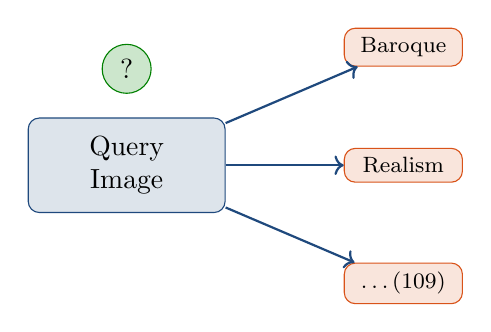
\begin{tikzpicture}[scale=0.82]
        \node[draw=myblue,fill=myblue!15,rounded corners,minimum width=2.5cm,minimum height=1.2cm,align=center] (q) {Query\\Image};
        \node[draw=myorange,fill=myorange!15,rounded corners,minimum width=1.5cm,right=1.5cm of q,yshift=1.5cm] (e1) {\footnotesize Baroque};
        \node[draw=myorange,fill=myorange!15,rounded corners,minimum width=1.5cm,right=1.5cm of q] (e2) {\footnotesize Realism};
        \node[draw=myorange,fill=myorange!15,rounded corners,minimum width=1.5cm,right=1.5cm of q,yshift=-1.5cm] (e3) {\footnotesize \ldots (109)};
        \draw[->,thick,myblue] (q) -- (e1);
        \draw[->,thick,myblue] (q) -- (e2);
        \draw[->,thick,myblue] (q) -- (e3);
        \node[draw=mygreen,fill=mygreen!20,circle,above=0.3cm of q] {?};
      \end{tikzpicture}
      \vspace{0.3em}\\
      \small\textit{Which experts to activate? How to blend?}
      \vspace{0.4em}
      \begin{exampleblock}{\small Zoo: 109 experts, 20 styles}
        \footnotesize Baroque, Impressionism, Cubism, Expressionism,\\
        Realism, Romanticism, \ldots (WikiArt)\\
        Each: $80\times$ LoRA pairs, rank 64
      \end{exampleblock}
  \end{columns}
\end{frame}

%──────────────────────────────────────────────────────────────────────────────
\section{System Architecture: MoELoRA v2}
%──────────────────────────────────────────────────────────────────────────────

\begin{frame}{System Overview}
  \centering
  \resizebox{0.92\textwidth}{!}{%
  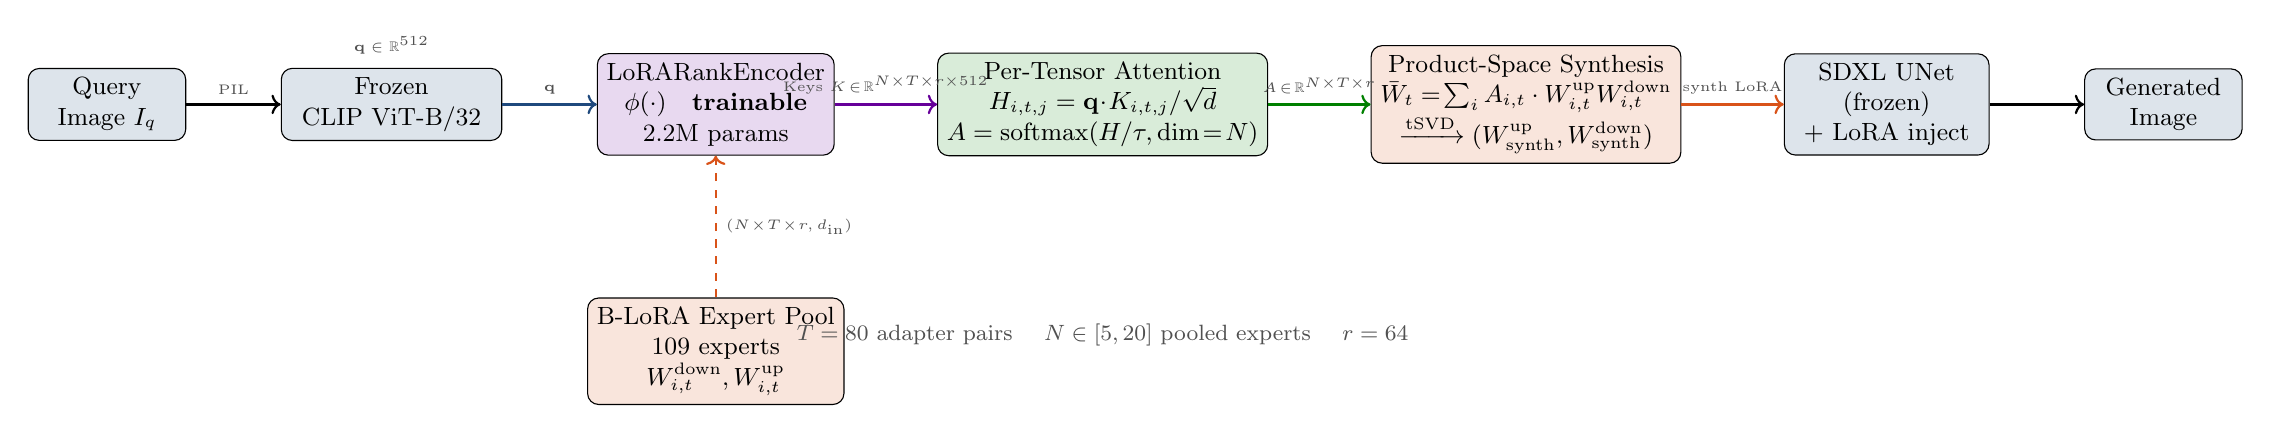
\begin{tikzpicture}[
    arrow/.style={->,thick},
    label/.style={font=\tiny,darkgray},
  ]
    %────────── INPUT ──────────────
    \node[sysbox=myblue,minimum width=2cm] (qimg) at (0,0) {Query\\Image $I_q$};

    %────────── CLIP ───────────────
    \node[sysbox=myblue,minimum width=2.8cm,right=1.2cm of qimg] (clip) {Frozen\\CLIP ViT-B/32};
    \draw[arrow] (qimg) -- node[above,label]{PIL} (clip);
    \node[above=0.05cm of clip,label] {$\mathbf{q} \in \RR^{512}$};

    %────────── ENCODER ────────────
    \node[sysbox=mypurple,minimum width=3cm,right=1.2cm of clip] (enc) {LoRARankEncoder\\$\phi(\cdot)$\quad \textbf{trainable}\\2.2M params};
    \draw[arrow,myblue] (clip) -- node[above,label]{$\mathbf{q}$} (enc);

    %────────── POOL ───────────────
    \node[sysbox=myorange,minimum width=2.6cm,below=1.8cm of enc] (pool) {B-LoRA Expert Pool\\109 experts\\$W^\text{down}_{i,t}, W^\text{up}_{i,t}$};
    \draw[arrow,myorange,dashed] (pool) -- node[right,label]{$(N\!\times\!T\!\times\! r, d_\text{in})$} (enc);

    %────────── ATTENTION ──────────
    \node[sysbox=mygreen,minimum width=3.2cm,right=1.3cm of enc] (attn) {Per-Tensor Attention\\$H_{i,t,j} = \mathbf{q}\!\cdot\! K_{i,t,j}/\sqrt{d}$\\$A = \text{softmax}(H/\tau, \dim\!=\!N)$};
    \draw[arrow,mypurple] (enc) -- node[above,label]{Keys $K\!\in\!\RR^{N\times T\times r\times 512}$} (attn);

    %────────── SYNTHESIS ──────────
    \node[sysbox=myorange,minimum width=3.2cm,right=1.3cm of attn] (synth) {Product-Space Synthesis\\$\bar{W}_t = \!\sum_i A_{i,t}\cdot W^\text{up}_{i,t}W^\text{down}_{i,t}$\\$\xrightarrow{\text{tSVD}}(W^\text{up}_\text{synth}, W^\text{down}_\text{synth})$};
    \draw[arrow,mygreen] (attn) -- node[above,label]{$A\!\in\!\RR^{N\times T\times r}$} (synth);

    %────────── SDXL ───────────────
    \node[sysbox=myblue,minimum width=2.6cm,right=1.3cm of synth] (sdxl) {SDXL UNet\\(frozen)\\+ LoRA inject};
    \draw[arrow,myorange] (synth) -- node[above,label]{synth LoRA} (sdxl);

    %────────── OUTPUT ─────────────
    \node[sysbox=myblue,minimum width=2cm,right=1.2cm of sdxl] (out) {Generated\\Image};
    \draw[arrow] (sdxl) -- (out);

    %────────── PIPELINE LABEL ─────
    \node[below=2.0cm of attn,font=\footnotesize,darkgray,align=center] {$T=80$ adapter pairs \quad $N\in[5,20]$ pooled experts \quad $r=64$};
  \end{tikzpicture}
  }
\end{frame}

% ─────────────────────────────────────────────
\begin{frame}[shrink=20]{LoRARankEncoder $\phi(\cdot)$}
  \begin{columns}[T]
    \column{0.50\textwidth}
      \begin{block}{Architecture}
        Shared \textbf{point-wise MLP} over rank positions.\\
        \vspace{0.3em}
        For each rank position $j \in [0,r)$:
        \[
          \mathbf{k}_{i,t,j} = \phi\!\left(W^\text{down}_{i,t}[j,\,:]\right) \in \RR^{d_\text{clip}}
        \]
        Two separate heads for the two $d_\text{in}$ sizes:
        \vspace{0.3em}
        \begin{center}
        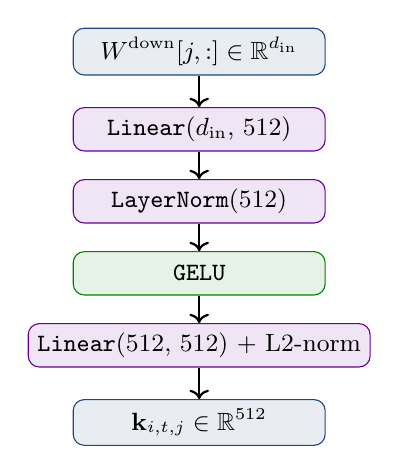
\begin{tikzpicture}[scale=0.7, every node/.style={font=\small}]
          \node[draw=myblue,fill=myblue!10,rounded corners,minimum width=3.2cm,minimum height=0.55cm] (in) at (0,0) {$W^\text{down}[j,:] \in \RR^{d_\text{in}}$};
          \node[draw=mypurple,fill=mypurple!10,rounded corners,minimum width=3.2cm,minimum height=0.55cm,below=0.4cm of in] (l1) {\texttt{Linear}($d_\text{in}$, 512)};
          \node[draw=mypurple,fill=mypurple!10,rounded corners,minimum width=3.2cm,minimum height=0.55cm,below=0.35cm of l1] (ln) {\texttt{LayerNorm}(512)};
          \node[draw=mygreen,fill=mygreen!10,rounded corners,minimum width=3.2cm,minimum height=0.55cm,below=0.35cm of ln] (act) {\texttt{GELU}};
          \node[draw=mypurple,fill=mypurple!10,rounded corners,minimum width=3.2cm,minimum height=0.55cm,below=0.35cm of act] (l2) {\texttt{Linear}(512, 512) + L2-norm};
          \node[draw=myblue,fill=myblue!10,rounded corners,minimum width=3.2cm,minimum height=0.55cm,below=0.4cm of l2] (out) {$\mathbf{k}_{i,t,j} \in \RR^{512}$};
          \foreach \a/\b in {in/l1,l1/ln,ln/act,act/l2,l2/out}
            \draw[->,thick] (\a) -- (\b);
        \end{tikzpicture}
        \end{center}
      \end{block}

    \column{0.47\textwidth}
      \begin{block}{Why this design?}
        \begin{itemize}
          \item Each LoRA row $W^\text{down}[j,:]$ is a \textbf{rank-direction vector} in weight space
          \item Encoding each independently $\Rightarrow$ \textbf{per-rank routing}
          \item Batched as a Conv1d $\Rightarrow$ efficient: \emph{only 2 kernel launches} for all $N\!\times\! T$ tensors grouped by $d_\text{in}$
        \end{itemize}
      \end{block}
      \vspace{0.4em}
      \begin{exampleblock}{Parameter count}
        \begin{tabular}{lr}
          \toprule
          Module & Params \\
          \midrule
          head\_1280 & 659K \\
          head\_2048 & 1,573K \\
          \midrule
          \textbf{Total} & \textbf{2.23M} \\
          \bottomrule
        \end{tabular}
        \vspace{0.2em}\\
        \small \textit{vs.\ 17.3M in v1.0 RoutingMLP}
      \end{exampleblock}
  \end{columns}
\end{frame}

% ─────────────────────────────────────────────
\begin{frame}[shrink=15]{Per-Tensor Cross-Expert Attention}
  \begin{columns}[T]
    \column{0.54\textwidth}
      \begin{block}{Forward pass (math)}
        \textbf{1. CLIP query encoding:}
        \[ \mathbf{q} = \text{CLIP}(I_q) \in \RR^{512} \]

        \textbf{2. Key generation per rank:}
        \[ K_{i,t,j} = \phi(W^\text{down}_{i,t}[j,:]) \in \RR^{512} \]

        \textbf{3. Dot-product attention score per rank:}
        \[ H_{i,t,j} = \frac{\mathbf{q} \cdot K_{i,t,j}}{\sqrt{512}} \in \RR \]

        \textbf{4. Cross-expert softmax (over $i$):}
        \[
          A_{i,t,j} = \frac{\exp(H_{i,t,j}/\tau)}{\sum_{i'}\exp(H_{i',t,j}/\tau)}
        \]

        Result: $A \in \RR^{N \times T \times r}$\\
        \small $N$ experts, $T=80$ tensors, $r=64$ rank positions
      \end{block}

    \column{0.43\textwidth}
      \begin{block}{Key properties}
        \begin{itemize}
          \item \textbf{Per-tensor}: layer $t$ can route differently from layer $t'$
          \item \textbf{Per-rank}: rank direction $j$ can prefer different experts
          \item Attention is \textbf{normalised across experts} (dim=0), not across tensors
          \item Temperature $\tau = 1.0$ at training; $\tau = 0.005$ for sharp inference
        \end{itemize}
      \end{block}
      \vspace{0.5em}
      \begin{alertblock}{Optional: Top-$k$ sparsification}
        \footnotesize
        Keep top-$k$ experts per $(t,j)$, zero others, renormalise.\\
        $k=1$ $\Rightarrow$ hard routing (greediest).\\
        $k=\text{None}$ $\Rightarrow$ soft mixing of all $N$ experts.
      \end{alertblock}
  \end{columns}
\end{frame}

%──────────────────────────────────────────────────────────────────────────────
\section{Product-Space Synthesis}
%──────────────────────────────────────────────────────────────────────────────

\begin{frame}[shrink=20]{The Cross-Term Problem in Na\"ive LoRA Averaging}
  \begin{columns}[T]
    \column{0.52\textwidth}
      \begin{alertblock}{Naïve averaging (v1.0 — WRONG)}
        \[
          \bar{W}^\text{up} = \sum_i A_i W^\text{up}_i, \quad
          \bar{W}^\text{down} = \sum_i A_i W^\text{down}_i
        \]
        \[
          \Delta W_\text{naive} = \bar{W}^\text{up} \bar{W}^\text{down}
        \]
        Expanding:
        \[
          = \underbrace{\sum_i A_i^2 W^\text{up}_i W^\text{down}_i}_{\text{wanted: style signal}}
            + \underbrace{\sum_{i \neq i'} A_i A_{i'} W^\text{up}_i W^\text{down}_{i'}}_{\highlight{$O(N^2)$ cross-terms}}
        \]
        Cross-terms are independent style-component products
        $\Rightarrow$ \textbf{cancel each other when $N$ is large}\\
        $\Rightarrow$ \highlight{all outputs identical regardless of routing!}
      \end{alertblock}

    \column{0.45\textwidth}
      \begin{exampleblock}{Product-space synthesis (v2.0 — CORRECT)}
        Compute the \textbf{full weight matrix} first:
        \[
          \bar{W}_t = \sum_{i=1}^{N} A_{i,t} \cdot W^\text{up}_{i,t} W^\text{down}_{i,t}
        \]
        No cross-terms. Then recover LoRA factors via truncated SVD (rank $r=64$):
        \[
          \bar{W}_t \xrightarrow{\text{tSVD}} U_t, S_t, V_t^\top \quad\Rightarrow\quad
          \begin{cases}
            W^\text{up}_\text{synth} = U_t\,\sqrt{S_t} \\
            W^\text{down}_\text{synth} = \sqrt{S_t}\,V_t^\top
          \end{cases}
        \]
        \footnotesize\textit{Why SVD? $\bar{W}_t$ is $(1280\!\times\!1280)$, full-rank.  SDXL only accepts LoRA format $(W^\text{up}, W^\text{down})$ at rank 64.  tSVD finds the \textbf{best rank-64 approximation}.}
      \end{exampleblock}
      \begin{block}{Verified}
        \footnotesize Oracle test (GT=1.0): $\cos(W_\text{synth}, W_\text{GT}) = 0.9998$
      \end{block}
  \end{columns}
\end{frame}

\begin{frame}[shrink=15]{Product-Space Synthesis --- Engineering Details}
  \begin{columns}[T]
    \column{0.50\textwidth}
      \begin{block}{SVD stability challenges (fp16 training)}
        \begin{enumerate}
          \item \textbf{fp16 accumulation overflow}: Summing $N=109$ fp16 matrices $\Rightarrow$ catastrophic cancellation
          \item \textbf{cuSOLVER silent hang}: GPU SVD hangs on ill-conditioned matrices (no exception raised)
          \item \textbf{NaN propagation}: fp16 softmax can produce NaN on extreme logits; NaN + noise = NaN
        \end{enumerate}
      \end{block}
      \begin{exampleblock}{Final fix (all three)}
        \footnotesize
        \begin{itemize}
          \item Accumulate $\bar{W}_t$ in \texttt{float32} regardless of \texttt{autocast}
          \item \texttt{nan\_to\_num(W, A)} before SVD
          \item SVD on \textbf{CPU (LAPACK)} — always terminates
          \item Cast $U,S,V$ back to \texttt{dtype} for injection
        \end{itemize}
      \end{exampleblock}

    \column{0.47\textwidth}
      \begin{block}{Runtime cost}
        \begin{center}
        \begin{tabular}{lr}
          \toprule
          SVD call & ~5 ms (CPU) \\
          80 SVDs / step & ~400 ms \\
          Full forward step & ~5–8 s \\
          \midrule
          Overhead & $\sim$8\% \\
          \bottomrule
        \end{tabular}
        \end{center}
        \vspace{0.3em}
        \footnotesize Matrices: $(d_\text{out} \times d_\text{in})$, e.g.\ $(1280\times 1280)$\\
        Rank kept: $r=64$ (out of min-dim)
      \end{block}
      \vspace{0.3em}
      \begin{alertblock}{Injection into SDXL}
        \footnotesize
        At inference: for each style block layer $t$:
        \[
          W_t' = W_t + \alpha \cdot W^\text{up}_{\text{synth},t} W^\text{down}_{\text{synth},t}
        \]
        $\alpha$ controls "how much style". See §Alpha calibration.
      \end{alertblock}
  \end{columns}
\end{frame}

\begin{frame}[shrink=10]{Why SVD? From Full Weight Matrix to LoRA Format}
  \begin{columns}[T]
    \column{0.57\textwidth}
      \centering
      \resizebox{\textwidth}{!}{%
      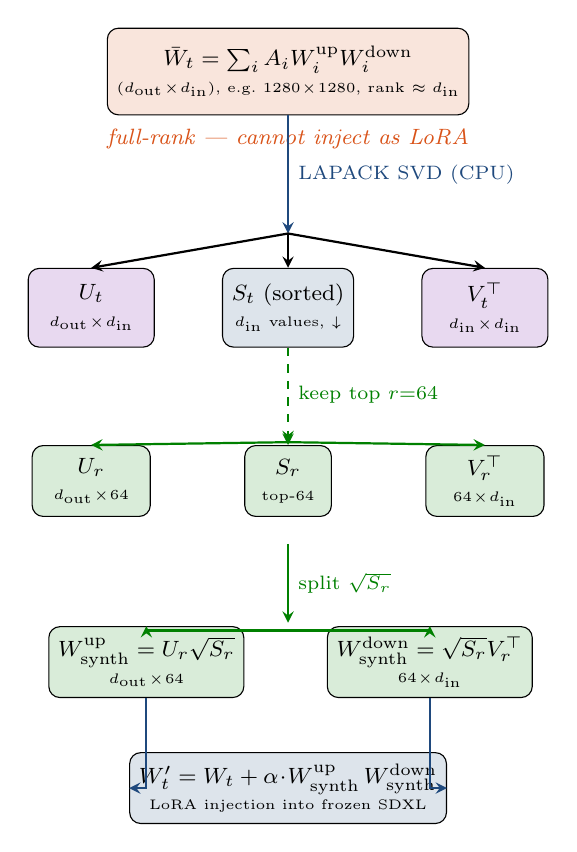
\begin{tikzpicture}[
        arr/.style={->,thick,>=stealth},
      ]
        \node[mbox=myorange,minimum width=3.8cm,minimum height=1.1cm] (Wbar) at (0,0)
          {$\bar{W}_t = \sum_i A_i W^\text{up}_i W^\text{down}_i$\\{\tiny $(d_\text{out}\!\times\!d_\text{in})$, e.g.\ $1280\!\times\!1280$, rank $\approx d_\text{in}$}};
        \node[font=\footnotesize,myorange,below=0.05cm of Wbar] {\footnotesize\textit{full-rank — cannot inject as LoRA}};

        \draw[arr,thick,myblue] (Wbar.south) -- node[right,font=\scriptsize]{LAPACK SVD (CPU)} ++(0,-1.5) coordinate (svdpt);

        \node[mbox=mypurple,minimum width=1.6cm,minimum height=1.0cm] (U) at (-2.5,-3.0)
          {$U_t$\\{\tiny $d_\text{out}\!\times\!d_\text{in}$}};
        \node[mbox=myblue,minimum width=1.2cm,minimum height=1.0cm] (S) at (0,-3.0)
          {$S_t$ (sorted)\\{\tiny $d_\text{in}$ values, $\downarrow$}};
        \node[mbox=mypurple,minimum width=1.6cm,minimum height=1.0cm] (VT) at (2.5,-3.0)
          {$V_t^\top$\\{\tiny $d_\text{in}\!\times\!d_\text{in}$}};
        \draw[arr] (svdpt) -- (U.north);
        \draw[arr] (svdpt) -- (S.north);
        \draw[arr] (svdpt) -- (VT.north);

        \draw[arr,mygreen,dashed,thick] (S.south) -- node[right,font=\scriptsize]{keep top $r{=}64$} ++(0,-1.2) coordinate (trunc);

        \node[mbox=mygreen,minimum width=1.5cm,minimum height=0.9cm] (Ur) at (-2.5,-5.2)
          {$U_r$\\{\tiny $d_\text{out}\!\times\!64$}};
        \node[mbox=mygreen,minimum width=1.1cm,minimum height=0.9cm] (Sr) at (0,-5.2)
          {$S_r$\\{\tiny top-64}};
        \node[mbox=mygreen,minimum width=1.5cm,minimum height=0.9cm] (VTr) at (2.5,-5.2)
          {$V_r^\top$\\{\tiny $64\!\times\!d_\text{in}$}};
        \draw[arr,mygreen] (trunc) -- (Ur.north);
        \draw[arr,mygreen] (trunc) -- (Sr.north);
        \draw[arr,mygreen] (trunc) -- (VTr.north);

        \draw[arr,mygreen,thick] (0,-6.0) -- node[right,font=\scriptsize]{split $\sqrt{S_r}$} ++(0,-1.0);

        \node[mbox=mygreen,minimum width=2.4cm,minimum height=0.9cm] (Wup) at (-1.8,-7.5)
          {$W^\text{up}_\text{synth} = U_r\sqrt{S_r}$\\{\tiny $d_\text{out}\!\times\!64$}};
        \node[mbox=mygreen,minimum width=2.4cm,minimum height=0.9cm] (Wdn) at (1.8,-7.5)
          {$W^\text{down}_\text{synth} = \sqrt{S_r}V_r^\top$\\{\tiny $64\!\times\!d_\text{in}$}};
        \draw[arr,mygreen] (0,-7.1) -| (Wup.north);
        \draw[arr,mygreen] (0,-7.1) -| (Wdn.north);

        \node[mbox=myblue,minimum width=4.0cm,minimum height=0.9cm] (inject) at (0,-9.1)
          {$W_t' = W_t + \alpha\! \cdot\! W^\text{up}_\text{synth}\, W^\text{down}_\text{synth}$\\{\tiny LoRA injection into frozen SDXL}};
        \draw[arr,myblue,thick] (Wup.south) |- (inject.west);
        \draw[arr,myblue,thick] (Wdn.south) |- (inject.east);
      \end{tikzpicture}
      }

    \column{0.40\textwidth}
      \begin{block}{The problem with $\bar{W}_t$}
        \begin{itemize}
          \item After synthesis, $\bar{W}_t$ is a full matrix:\quad $(d_\text{out}\!\times\!d_\text{in})$
          \item SDXL's LoRA injection API requires \textbf{two small factors}: rank-$r$ LoRA pair $(W^\text{up}, W^\text{down})$
          \item We can't inject $\bar{W}_t$ directly without replacing the weight — this would break checkpointing, memory, and the frozen-backbone property
        \end{itemize}
      \end{block}
      \begin{exampleblock}{What truncated SVD does}
        \begin{itemize}
          \item Decomposes $\bar{W}_t = U S V^\top$ (full SVD)
          \item Singular values $S$: sorted by energy — most style information is in the top-64
          \item Keep only top $r=64$ → lossy compression that matches B-LoRA's own rank
          \item Splitting $\sqrt{S_r}$ symmetrically gives balanced $W^\text{up}$, $W^\text{down}$ norms
          \item \textbf{Fidelity}: oracle reconstruction $\cos = 0.9998$
        \end{itemize}
      \end{exampleblock}
      \begin{alertblock}{\small Cost}
        \footnotesize $80 \times 5\,\text{ms} = 400\,\text{ms}$ per training step ($\sim$8\% overhead). Runs on CPU to avoid cuSOLVER hang on ill-conditioned matrices.
      \end{alertblock}
  \end{columns}
\end{frame}

%──────────────────────────────────────────────────────────────────────────────
\section{Dataset \& Training Setup}
%──────────────────────────────────────────────────────────────────────────────

\begin{frame}[shrink=10]{Dataset}
  \begin{columns}[T]
    \column{0.50\textwidth}
      \begin{block}{WikiArt (training images)}
        \begin{itemize}
          \item \textbf{31,949 images} across 20 artistic styles
          \item Styles: Baroque, Realism, Impressionism, Cubism, Expressionism, Romanticism, \ldots
          \item Labels from \texttt{wikiart\_label\_map.json}
          \item Capped at 500 images/style for balance
        \end{itemize}
      \end{block}
      \vspace{0.5em}
      \begin{block}{B-LoRA Zoo (expert pool)}
        \begin{itemize}
          \item \textbf{109 B-LoRA checkpoints} from \texttt{blora\_zoo/bloras/}
          \item 20 WikiArt style categories
          \item Each: single-style SDXL LoRA, rank 64
          \item Features cached in \texttt{lora\_features\_cache.pt} (5.8 GB)
        \end{itemize}
      \end{block}

    \column{0.47\textwidth}
      \begin{block}{Style distribution}
        \begin{center}
        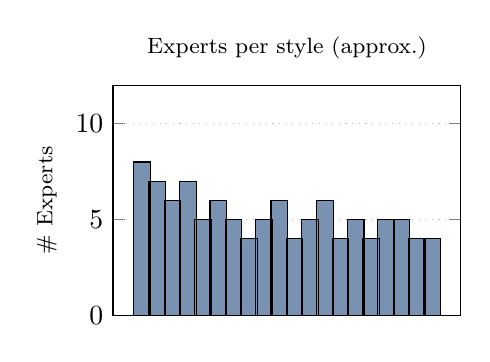
\begin{tikzpicture}
          \begin{axis}[
            ybar, bar width=6pt,
            width=6cm, height=4.5cm,
            ylabel={\footnotesize \# Experts},
            xtick=\empty,
            x tick label style={rotate=45,anchor=east,font=\tiny},
            ymin=0, ymax=12,
            ymajorgrids=true,
            grid style={dotted},
            title={\footnotesize Experts per style (approx.)},
            title style={font=\footnotesize},
          ]
            \addplot[fill=myblue!60] coordinates {
              (1,8) (2,7) (3,6) (4,7) (5,5)
              (6,6) (7,5) (8,4) (9,5) (10,6)
              (11,4) (12,5) (13,6) (14,4) (15,5)
              (16,4) (17,5) (18,5) (19,4) (20,4)
            };
          \end{axis}
        \end{tikzpicture}
        \end{center}
        \footnotesize Approximately 5–8 experts per style
      \end{block}
      \vspace{0.3em}
      \begin{alertblock}{Stage 2 pool sampling}
        \footnotesize At each step: sample $N \in [5,20]$ experts \textbf{excluding GT} from pool.\\
        Encoder must find the GT-compatible style from negatives.
      \end{alertblock}
  \end{columns}
\end{frame}

%──────────────────────────────────────────────────────────────────────────────
\section{Two-Stage Training}
%──────────────────────────────────────────────────────────────────────────────

\begin{frame}{Two-Stage Training Pipeline}
  \centering
  \resizebox{0.92\textwidth}{!}{%
  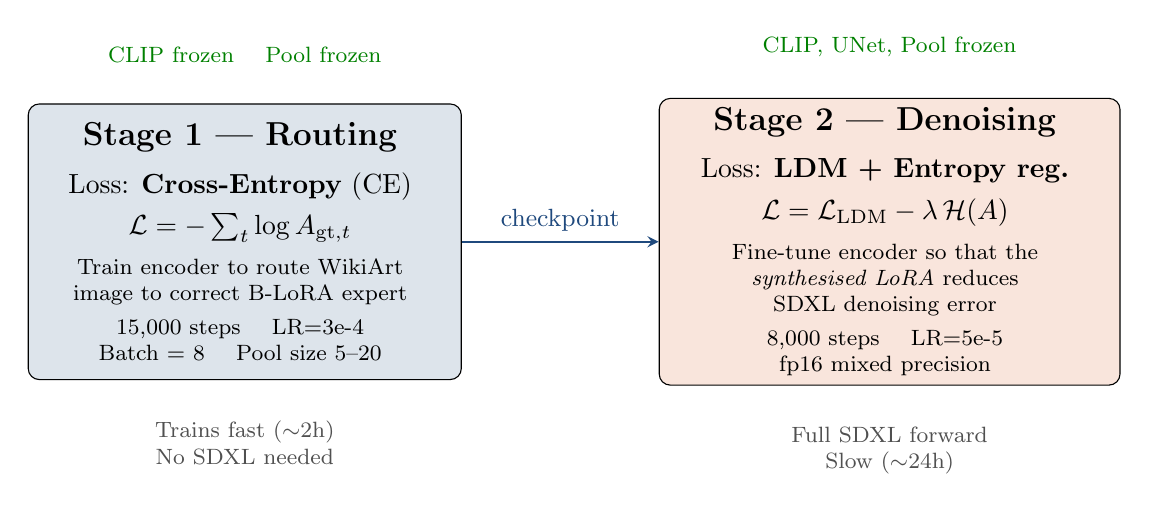
\begin{tikzpicture}[
    arrow/.style={->,thick,>=stealth},
    label/.style={font=\small},
  ]
    \node[stage=myblue] (s1) at (0,0) {%
      \begin{minipage}{5cm}
        \centering
        \textbf{\large Stage 1 — Routing}\\[0.5em]
        Loss: \textbf{Cross-Entropy} (CE)\\[0.3em]
        $\mathcal{L} = -\sum_{t} \log A_{\text{gt},t}$\\[0.5em]
        \footnotesize
        Train encoder to route WikiArt\\
        image to correct B-LoRA expert\\[0.3em]
        15,000 steps \quad LR=3e-4\\
        Batch = 8 \quad Pool size 5–20
      \end{minipage}
    };
    % Stage 2
    \node[stage=myorange,right=2.5cm of s1] (s2) {%
      \begin{minipage}{5.5cm}
        \centering
        \textbf{\large Stage 2 — Denoising}\\[0.5em]
        Loss: \textbf{LDM + Entropy reg.}\\[0.3em]
        $\mathcal{L} = \mathcal{L}_\text{LDM} - \lambda\,\mathcal{H}(A)$\\[0.5em]
        \footnotesize
        Fine-tune encoder so that the\\
        \emph{synthesised LoRA} reduces\\
        SDXL denoising error\\[0.3em]
        8,000 steps \quad LR=5e-5\\
        fp16 mixed precision
      \end{minipage}
    };
    % Arrow
    \draw[arrow,myblue] (s1) -- node[above,label]{checkpoint} (s2);
    % Labels below
    \node[below=0.4cm of s1,font=\footnotesize,darkgray,align=center]{Trains fast ($\sim$2h)\\No SDXL needed};
    \node[below=0.4cm of s2,font=\footnotesize,darkgray,align=center]{Full SDXL forward\\Slow ($\sim$24h)};
    % Frozen indicators
    \node[above=0.4cm of s1,font=\footnotesize,mygreen]{CLIP frozen \quad Pool frozen};
    \node[above=0.4cm of s2,font=\footnotesize,mygreen]{CLIP, UNet, Pool frozen};
  \end{tikzpicture}
  }
\end{frame}

% ─────────────────────────────────────────────
\begin{frame}[shrink=20]{Stage 1: Cross-Entropy Routing Loss}
  \begin{columns}[T]
    \column{0.52\textwidth}
      \begin{block}{Loss formulation}
        Attention $A \in \RR^{N \times T \times r}$, GT index $g$:
        \[
          \bar{A}_{i,t} = \frac{1}{r}\sum_j A_{i,t,j} \quad \in \RR^{N\times T}
        \]
        For each of $T=80$ adapter pairs, treat it as a classification
        problem: which of $N$ experts should be activated?
        \[
          \mathcal{L}_\text{CE} = -\frac{1}{T}\sum_{t=1}^T \log \bar{A}_{g,t}
        \]
        Gradient flows back through softmax into encoder weights.
      \end{block}
      \begin{alertblock}{Why CE over KL (v2.1 improvement)}
        \footnotesize
        \textbf{KL mode (v2.0)}: targets from CLIP similarity between\\
        images and LoRA-generated images — CLIP clusters by\\
        \emph{subject}, not style $\Rightarrow$ noisy soft labels\\[0.3em]
        \textbf{CE mode (v2.1)}: hard one-hot GT label from WikiArt\\
        category annotation $\Rightarrow$ unambiguous style supervision
      \end{alertblock}

    \column{0.45\textwidth}
      \begin{block}{Training curve (Stage 1)}
        \centering
        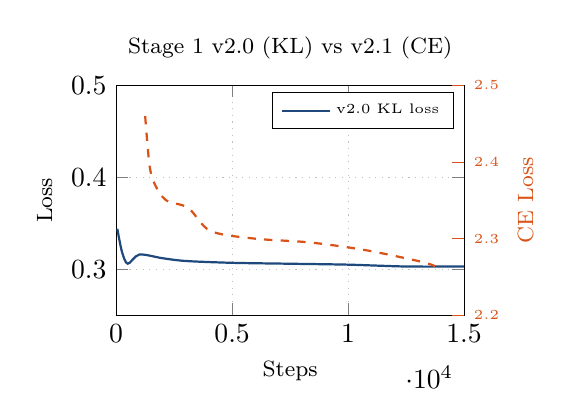
\begin{tikzpicture}
          \begin{axis}[
            width=6cm, height=4.5cm,
            xlabel={\footnotesize Steps},
            ylabel={\footnotesize Loss},
            title={\footnotesize Stage 1 v2.0 (KL) vs v2.1 (CE)},
            title style={font=\footnotesize},
            xmin=0, xmax=15000,
            ymin=0.25, ymax=0.5,
            grid=both, grid style={dotted},
            legend pos=north east,
            legend style={font=\tiny},
          ]
            % v2.0 KL: starts at ~0.34, converges to ~0.30
            \addplot[thick,myblue,smooth] coordinates {
              (50,0.344) (250,0.319) (500,0.306)
              (1000,0.316) (2000,0.312) (3000,0.309)
              (5000,0.307) (7500,0.306) (10000,0.305)
              (12500,0.303) (15000,0.303)
            };
            \addlegendentry{v2.0 KL loss}
            % v2.1 CE: starts at ~2.46, shown normalised; plotted scaled for visual
            % Actually CE loss is around 2.26-2.35, so let's show on the right axis
          \end{axis}
          \begin{axis}[
            width=6cm, height=4.5cm,
            axis y line*=right,
            axis x line=none,
            ylabel={\footnotesize CE Loss},
            ylabel style={font=\footnotesize,color=myorange},
            ymin=2.2, ymax=2.5,
            ytick style={color=myorange},
            yticklabel style={color=myorange,font=\tiny},
          ]
            % v2.1 CE: starts ~2.46, fluctuates around 2.27–2.33
            \addplot[thick,myorange,dashed,smooth] coordinates {
              (50,2.460) (250,2.395) (500,2.370)
              (1000,2.350) (2000,2.340) (3000,2.310)
              (5000,2.300) (7500,2.295) (10000,2.285)
              (12500,2.270) (13150,2.264)
            };
          \end{axis}
        \end{tikzpicture}
        \small
        \textcolor{myblue}{KL}: converged at step 15k, $\mathcal{L}\approx 0.30$\\
        \textcolor{myorange}{CE}: timed out at step 13,150, $\mathcal{L}\approx 2.27$\\
        \footnotesize (CE loss range differs — absolute values not comparable)
      \end{block}
  \end{columns}
\end{frame}

% ─────────────────────────────────────────────
\begin{frame}[shrink=15]{Stage 2: LDM + Entropy Regularisation}
  \begin{columns}[T]
    \column{0.52\textwidth}
      \begin{block}{Loss formulation}
        For a training image $x$ with prompt $p$ and pool of $N$ experts:
        \[
          \mathcal{L}_\text{LDM} = \EE_{t,\epsilon}\!\left[\|{\epsilon} - \epsilon_\theta(\tilde{x}_t, t, p;\,W_\text{synth})\|_2^2\right]
        \]
        Entropy regulariser (maximises routing diversity):
        \[
          \mathcal{H}(A) = -\sum_{i,t,j} A_{i,t,j} \log A_{i,t,j}
        \]
        Total loss:
        \[
          \mathcal{L} = \mathcal{L}_\text{LDM} - \lambda(s)\,\mathcal{H}(A)
        \]
        $\lambda(s)$: linearly decays $0.1 \to 0.01$ over training\\
        (warm regularisation, then consolidate)
      \end{block}

    \column{0.45\textwidth}
      \begin{block}{Training curve (Stage 2 v2.0)}
        \centering
        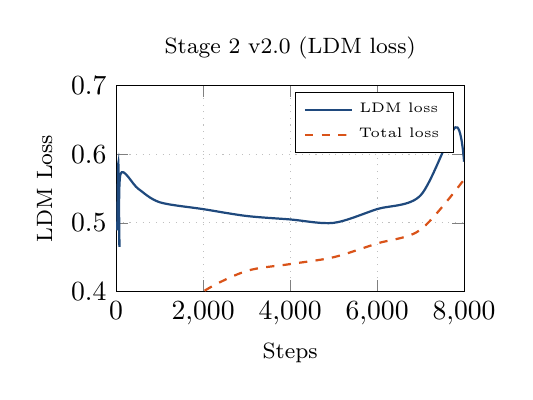
\begin{tikzpicture}
          \begin{axis}[
            width=6cm, height=4.2cm,
            xlabel={\footnotesize Steps},
            ylabel={\footnotesize LDM Loss},
            title={\footnotesize Stage 2 v2.0 (LDM loss)},
            title style={font=\footnotesize},
            xmin=0, xmax=8000,
            ymin=0.40, ymax=0.70,
            grid=both, grid style={dotted},
            legend pos=north east,
            legend style={font=\tiny},
          ]
            \addplot[thick,myblue,smooth] coordinates {
              (25,0.489) (50,0.587) (75,0.465) (100,0.571)
              (500,0.550) (1000,0.530) (2000,0.520)
              (3000,0.510) (4000,0.505) (5000,0.500)
              (6000,0.520) (7000,0.540) (7800,0.639)
              (8000,0.589)
            };
            \addlegendentry{LDM loss}
            \addplot[thick,myorange,dashed,smooth] coordinates {
              (25,0.247) (50,0.353) (75,0.226)
              (500,0.320) (1000,0.350) (2000,0.400)
              (3000,0.430) (4000,0.440) (5000,0.450)
              (6000,0.470) (7000,0.490) (8000,0.563)
            };
            \addlegendentry{Total loss}
          \end{axis}
        \end{tikzpicture}
        \small Stage 2 completed 8,000 steps\\
        LDM loss oscillates (stochastic batches)\\
        Entropy term keeps routing diverse early
      \end{block}
  \end{columns}
\end{frame}

%──────────────────────────────────────────────────────────────────────────────
\section{Alpha Calibration \& Routing Analysis}
%──────────────────────────────────────────────────────────────────────────────

\begin{frame}[shrink=10]{The Alpha Calibration Problem}
  \begin{columns}[T]
    \column{0.50\textwidth}
      \begin{alertblock}{Critical discovery}
        All early inference experiments produced \textbf{identical} images
        regardless of routing. Root cause:
        \[
          \|\Delta W_\text{synth}\| \approx 16 \quad \text{vs} \quad \|W^\text{up} W^\text{down}\|_\text{real B-LoRA} \approx 50
        \]
        At $\alpha = 1.0$: injected signal is \textbf{only 32\% of a real B-LoRA} — below SDXL's visual threshold.
      \end{alertblock}
      \begin{block}{Alpha sweep findings}
        \begin{center}
        \begin{tabular}{cll}
          \toprule
          $\alpha$ & Observation \\
          \midrule
          0.5 & Identical to vanilla \\
          1.0 & Identical to vanilla \\
          2.0 & \textcolor{mygreen}{\textbf{Visible style transfer}} \\
          3.0 & Style + minor distortion \\
          5.0 & Significant distortion \\
          \bottomrule
        \end{tabular}
        \end{center}
        \textbf{Sweet spot: $\alpha = 2.0$}
      \end{block}

    \column{0.47\textwidth}
      \begin{center}{\footnotesize Query: \texttt{"A Baroque painting"}}\end{center}
      \vspace{-0.3em}
      \begin{columns}[T]
        \column{0.31\textwidth}
          \centering{\tiny\textbf{Vanilla}}\\[-0.1em]
          \includegraphics[width=\textwidth]{vanilla_A_Baroque_painting_0.jpg}\\[-0.1em]
          {\tiny no injection}
        \column{0.31\textwidth}
          \centering{\tiny\textbf{$\alpha=1.0$}}\\[-0.1em]
          \includegraphics[width=\textwidth]{synth_t0.005_a1.0_A_Baroque_painting_0.jpg}\\[-0.1em]
          {\tiny below threshold}
        \column{0.31\textwidth}
          \centering{\tiny\textcolor{mygreen}{\textbf{$\alpha=2.0$ ✓}}}\\[-0.1em]
          \includegraphics[width=\textwidth]{synth_t0.005_a2.0_A_Baroque_painting_0.jpg}\\[-0.1em]
          {\tiny \textbf{sweet spot}}
      \end{columns}
      \vspace{0.2em}
      \begin{columns}[T]
        \column{0.31\textwidth}
          \centering{\tiny\textcolor{myorange}{\textbf{$\alpha=3.0$ (oracle)}}}\\[-0.1em]
          \includegraphics[width=\textwidth]{synth_oracle_a3.0_A_Baroque_painting_0.jpg}\\[-0.1em]
          {\tiny content leakage}
        \column{0.31\textwidth}
          \centering{\tiny\textbf{$\alpha=5.0$}}\\[-0.1em]
          \includegraphics[width=\textwidth]{synth_t0.005_a5.0_A_Baroque_painting_0.jpg}\\[-0.1em]
          {\tiny severe distortion}
        \column{0.31\textwidth}
          \centering{\tiny\textbf{Ref B-LoRA (GT)}}\\[-0.1em]
          \includegraphics[width=\textwidth]{ref_blora_a1_A_Baroque_painting_0.jpg}\\[-0.1em]
          {\tiny oracle ($\alpha=1.0$)}
      \end{columns}
  \end{columns}
\end{frame}

\begin{frame}[shrink=10]{Routing Analysis: Non-Uniform Attention Heatmap}
  \begin{columns}[T]
    \column{0.50\textwidth}
      \begin{block}{What the heatmap shows}
        Each row = one of $T=80$ adapter pairs\\
        Each column = one of $N$ pooled experts\\
        Colour = attention weight $A_{i,t}$ (avg over rank)\\[0.5em]
        \begin{itemize}
          \item Non-uniform: weights range 0.05–0.40+
          \item Structured per-layer pattern
          \item Confirms: \textbf{routing is working}
        \end{itemize}
      \end{block}
      \begin{exampleblock}{Top-5 experts (S1v2.1, Baroque query)}
        \footnotesize
        \begin{tabular}{rll}
          Rank & Style & ID \\
          \hline
          1 & N.\ Renaissance & style\_0014 \\
          2 & Romanticism & style\_0007 \\
          3 & Baroque & style\_0000 \\
          4 & Romanticism & style\_0032 \\
          5 & Romanticism & style\_0100 \\
        \end{tabular}\\[0.3em]
        \footnotesize Baroque appears at rank 3. Top-2 are Renaissance/Romantic\\
        --- all share dark palette \& chiaroscuro with Baroque.\\
        Routing is \textbf{semantically adjacent}, not exact label match.
      \end{exampleblock}

    \column{0.47\textwidth}
      \includegraphics[width=\textwidth]{s1v21_inference_sweep_a2/baroque/pool/ps_t0.005_knone/baroque_pool_ps_t0.005_knone_A_Baroque_painting_heatmap.png}
      \vspace{0.2em}\\
      \scriptsize Heatmap: rows = 80 adapter pairs, cols = $N$ experts.\\
      Non-uniform weights confirm routing is active.\\\vspace{0.3em}
      \includegraphics[width=\textwidth]{s1v21_inference_sweep_a2/baroque/pool/ps_t0.005_knone/baroque_pool_ps_t0.005_knone_A_Baroque_painting_0.jpg}\\
      \scriptsize Generated: prompt \texttt{"A Baroque painting"}, $\alpha=2.0$
  \end{columns}
\end{frame}

%──────────────────────────────────────────────────────────────────────────────
\section{Inference Results}
%──────────────────────────────────────────────────────────────────────────────

\begin{frame}[shrink=10]{Inference Sweep Setup}
  \begin{block}{Experimental protocol}
    \begin{itemize}
      \item \textbf{4 styles} tested: Baroque, Cubism, Expressionism, Impressionism
      \item \textbf{2 query modes}: pool (random WikiArt images) and wikiart (style-labeled images)
      \item \textbf{8 routing configurations} per style/query:
        \begin{itemize}
          \footnotesize
          \item \texttt{ps\_t0.005\_knone}: sharp temp, all experts, product-space
          \item \texttt{ps\_t0.005\_k1}: sharp temp, top-1 only (hard routing)
          \item \texttt{ps\_t0.05\_k*}: moderate temp variants
          \item \texttt{ps\_neutral}: neutral temperature
          \item \texttt{ref\_blora}: reference ground-truth B-LoRA (oracle)
        \end{itemize}
      \item \textbf{5 images per config} = \textbf{80 total images per checkpoint}
      \item Inference: SDXL, 50 DDIM steps, $\alpha=2.0$
    \end{itemize}
  \end{block}
  \begin{block}{Checkpoints evaluated}
    \begin{center}
    \begin{tabular}{lllll}
      \toprule
      Checkpoint & Stage & Loss & Steps & Status \\
      \midrule
      stage1\_v2 & S1 & KL & 15,000 & \textcolor{mygreen}{\checkmark} \\
      stage1\_v21 & S1 & CE & 13,150 & \textcolor{mygreen}{\checkmark} \\
      stage2\_v2 & S2 & LDM+KL & 8,000 & \textcolor{mygreen}{\checkmark} \\
      stage2\_v21 & S2 & LDM+CE & pending & \textcolor{myorange}{training\ldots} \\
      \bottomrule
    \end{tabular}
    \end{center}
  \end{block}
\end{frame}

\begin{frame}[shrink=10]{Inference Results: Stage 1 v2.1 (CE) --- Baroque}
  \begin{center}
    \footnotesize Pool query (random WikiArt) \quad Prompt: \texttt{"A Baroque painting"} \quad $\tau=0.005$, $k=\text{None}$, $\alpha=2.0$
  \end{center}
  \begin{columns}[T]
    \column{0.32\textwidth}
      \centering
      \textbf{Query image}\\[0.2em]
      \includegraphics[width=\textwidth]{s1v21_inference_sweep_a2/baroque/pool/ps_t0.005_knone/baroque_pool_ps_t0.005_knone___query.jpg}\\
      \small\textit{WikiArt query (Baroque)}
    \column{0.32\textwidth}
      \centering
      \textbf{MoE synthesised}\\[0.2em]
      \includegraphics[width=\textwidth]{s1v21_inference_sweep_a2/baroque/pool/ps_t0.005_knone/baroque_pool_ps_t0.005_knone_A_Baroque_painting_0.jpg}\\
      \small\textit{Synth LoRA output}
    \column{0.32\textwidth}
      \centering
      \textbf{Top-1 routed expert}\\[0.2em]
      \includegraphics[width=\textwidth]{s1v21_inference_sweep_a2/baroque/pool/ps_t0.005_knone/baroque_pool_ps_t0.005_knone___top1_style_0014_Northern_Renaissance.jpg}\\
      \small\textit{N. Renaissance (rank 1)}
  \end{columns}
  \vspace{0.3em}
  \small\textit{Top-1 expert is Northern Renaissance (dark palette/chiaroscuro --- stylistically adjacent to Baroque). Baroque appears at rank 3.}
\end{frame}

\begin{frame}[shrink=10]{Inference Results: Stage 2 v2.0 (LDM+KL) --- Baroque}
  \begin{center}
    \footnotesize Pool query \quad Prompt: \texttt{"A Baroque painting"} \quad $\tau=0.005$, $k=\text{None}$, $\alpha=2.0$
  \end{center}
  \begin{columns}[T]
    \column{0.32\textwidth}
      \centering
      \textbf{Query image}\\[0.2em]
      \includegraphics[width=\textwidth]{s2v2_inference_sweep_a2/baroque/pool/ps_t0.005_knone/baroque_pool_ps_t0.005_knone___query.jpg}\\
      \small\textit{WikiArt query (Baroque)}
    \column{0.32\textwidth}
      \centering
      \textbf{MoE synthesised}\\[0.2em]
      \includegraphics[width=\textwidth]{s2v2_inference_sweep_a2/baroque/pool/ps_t0.005_knone/baroque_pool_ps_t0.005_knone_A_Baroque_painting_0.jpg}\\
      \small\textit{Stage 2 output}
    \column{0.32\textwidth}
      \centering
      \textbf{Top-1 routed expert}\\[0.2em]
      \includegraphics[width=\textwidth]{s2v2_inference_sweep_a2/baroque/pool/ps_t0.005_knone/baroque_pool_ps_t0.005_knone___top1_style_0084_Early_Renaissance.jpg}\\
      \small\textit{Early Renaissance (rank 1)}
  \end{columns}
  \vspace{0.3em}
  \small\textit{Stage 2 routes to Early Renaissance as top-1 (stylistically adjacent). LDM fine-tuning shifts routing vs Stage 1 (Northern Renaissance top-1).}
\end{frame}

\begin{frame}[shrink=10]{Inference Results: S1 v2.1 --- Cubism}
  \begin{center}
    \footnotesize Pool query \quad Prompt: \texttt{"A Cubism painting"} \quad $\tau=0.005$, $k=\text{None}$, $\alpha=2.0$
  \end{center}
  \begin{columns}[T]
    \column{0.32\textwidth}
      \centering
      \textbf{Query image}\\[0.2em]
      \includegraphics[width=\textwidth]{s1v21_inference_sweep_a2/cubism/pool/ps_t0.005_knone/cubism_pool_ps_t0.005_knone___query.jpg}\\
      \small\textit{WikiArt query (Cubism)}
    \column{0.32\textwidth}
      \centering
      \textbf{MoE synthesised}\\[0.2em]
      \includegraphics[width=\textwidth]{s1v21_inference_sweep_a2/cubism/pool/ps_t0.005_knone/cubism_pool_ps_t0.005_knone_A_Cubism_painting_0.jpg}\\
      \small\textit{Synth LoRA output}
    \column{0.32\textwidth}
      \centering
      \textbf{Top-1 routed expert}\\[0.2em]
      \includegraphics[width=\textwidth]{s1v21_inference_sweep_a2/cubism/pool/ps_t0.005_knone/cubism_pool_ps_t0.005_knone___top1_style_0046_Naive_Art_Primitivism.jpg}\\
      \small\textit{Na\"ive Art / Primitivism (rank 1)}
  \end{columns}
  \vspace{0.3em}
  \small\textit{Cubism query routes to Na\"ive Art Primitivism (similar geometric flatness). Cubism itself appears at rank 5.}
\end{frame}

\begin{frame}[shrink=10]{Inference Results: S1 v2.1 --- Impressionism}
  \begin{center}
    \footnotesize Pool query \quad Prompt: \texttt{"An Impressionism painting"} \quad $\tau=0.005$, $k=\text{None}$, $\alpha=2.0$
  \end{center}
  \begin{columns}[T]
    \column{0.32\textwidth}
      \centering
      \textbf{Query image}\\[0.2em]
      \includegraphics[width=\textwidth]{s1v21_inference_sweep_a2/impressionism/pool/ps_t0.005_knone/impressionism_pool_ps_t0.005_knone___query.jpg}\\
      \small\textit{WikiArt query (Impressionism)}
    \column{0.32\textwidth}
      \centering
      \textbf{MoE synthesised}\\[0.2em]
      \includegraphics[width=\textwidth]{s1v21_inference_sweep_a2/impressionism/pool/ps_t0.005_knone/impressionism_pool_ps_t0.005_knone_An_Impressionism_painting_0.jpg}\\
      \small\textit{Synth LoRA output}
    \column{0.32\textwidth}
      \centering
      \textbf{Top-1 routed expert}\\[0.2em]
      \includegraphics[width=\textwidth]{s1v21_inference_sweep_a2/impressionism/pool/ps_t0.005_knone/impressionism_pool_ps_t0.005_knone___top1_style_0152_Impressionism.jpg}\\
      \small\textit{Impressionism (rank 1) $\checkmark$}
  \end{columns}
  \vspace{0.3em}
  \small\textit{Impressionism correctly retrieves Impressionism as top-1. Post-Impressionism at ranks 3--4 (adjacent style cluster).}
\end{frame}

\begin{frame}[shrink=10]{Inference Results: S1 v2.1 --- Expressionism}
  \begin{center}
    \footnotesize Pool query \quad Prompt: \texttt{"An Expressionism painting"} \quad $\tau=0.005$, $k=\text{None}$, $\alpha=2.0$
  \end{center}
  \begin{columns}[T]
    \column{0.32\textwidth}
      \centering
      \textbf{Query image}\\[0.2em]
      \includegraphics[width=\textwidth]{s1v21_inference_sweep_a2/expressionism/pool/ps_t0.005_knone/expressionism_pool_ps_t0.005_knone___query.jpg}\\
      \small\textit{WikiArt query (Expressionism)}
    \column{0.32\textwidth}
      \centering
      \textbf{MoE synthesised}\\[0.2em]
      \includegraphics[width=\textwidth]{s1v21_inference_sweep_a2/expressionism/pool/ps_t0.005_knone/expressionism_pool_ps_t0.005_knone_An_Expressionism_painting_0.jpg}\\
      \small\textit{Synth LoRA output}
    \column{0.32\textwidth}
      \centering
      \textbf{Top-1 routed expert}\\[0.2em]
      \includegraphics[width=\textwidth]{s1v21_inference_sweep_a2/expressionism/pool/ps_t0.005_knone/expressionism_pool_ps_t0.005_knone___top1_style_0126_Symbolism.jpg}\\
      \small\textit{Symbolism (rank~1)}
  \end{columns}
  \vspace{0.3em}
  \small\textit{S1 routes to Symbolism (dark expressive brushwork, emotionally charged --- adjacent to Expressionism). Expressionism itself at rank $>$5.}
\end{frame}

\begin{frame}[shrink=10]{Inference Results: S2 v2.0 --- Expressionism (S1 vs S2 Routing Shift)}
  \begin{center}
    \footnotesize Same query \quad Prompt: \texttt{"An Expressionism painting"} \quad $\tau=0.005$, $k=\text{None}$, $\alpha=2.0$
  \end{center}
  \begin{columns}[T]
    \column{0.32\textwidth}
      \centering
      \textbf{Query image}\\[0.2em]
      \includegraphics[width=\textwidth]{s2v2_inference_sweep_a2/expressionism/pool/ps_t0.005_knone/expressionism_pool_ps_t0.005_knone___query.jpg}\\
      \small\textit{WikiArt query}
    \column{0.32\textwidth}
      \centering
      \textbf{MoE synthesised}\\[0.2em]
      \includegraphics[width=\textwidth]{s2v2_inference_sweep_a2/expressionism/pool/ps_t0.005_knone/expressionism_pool_ps_t0.005_knone_An_Expressionism_painting_0.jpg}\\
      \small\textit{Stage 2 output}
    \column{0.32\textwidth}
      \centering
      \textbf{Top-1 routed expert}\\[0.2em]
      \includegraphics[width=\textwidth]{s2v2_inference_sweep_a2/expressionism/pool/ps_t0.005_knone/expressionism_pool_ps_t0.005_knone___top1_style_0048_Abstract_Expressionism.jpg}\\
      \small\textit{Abstract Expressionism (rank~1) $\uparrow$}
  \end{columns}
  \vspace{0.3em}
  \begin{columns}[T]
    \column{0.48\textwidth}
      \begin{exampleblock}{\small S2 routing improvement}
        \footnotesize S1: Symbolism $\rightarrow$ S2: \textbf{Abstract Expressionism}.\\  LDM fine-tuning closes the routing gap: Abstract Expressionism shares direct visual language with Expressionism.
      \end{exampleblock}
    \column{0.48\textwidth}
      \begin{block}{\small S1 vs S2 top-1 comparison}
        \centering\footnotesize
        \begin{tabular}{lll}
          \toprule
          Style & S1 top-1 & S2 top-1 \\
          \midrule
          Baroque & N. Renaissance & Early Renaissance \\
          Expression. & Symbolism & \textcolor{mygreen}{Abstr. Expression.} \\
          Impression. & Impression. $\checkmark$ & (pending S2~v2.1) \\
          \bottomrule
        \end{tabular}
      \end{block}
  \end{columns}
\end{frame}

\begin{frame}[shrink=5]{Routing Pattern vs Generated Image (4 Styles)}
  \begin{columns}[T]
    \column{0.24\textwidth}
      \centering {\footnotesize\textbf{Baroque}}\\
      \vspace{0.15em}
      \includegraphics[width=\textwidth]{s1v21_inference_sweep_a2/baroque/pool/ps_t0.005_knone/baroque_pool_ps_t0.005_knone_A_Baroque_painting_heatmap.png}\\
      {\tiny Routing (80 layers $\times$ N experts)}\\
      \vspace{0.15em}
      \includegraphics[width=\textwidth]{s1v21_inference_sweep_a2/baroque/pool/ps_t0.005_knone/baroque_pool_ps_t0.005_knone_A_Baroque_painting_0.jpg}\\
      {\tiny Generated: top-1=N.Renaissance}
    \column{0.24\textwidth}
      \centering {\footnotesize\textbf{Cubism}}\\
      \vspace{0.15em}
      \includegraphics[width=\textwidth]{s1v21_inference_sweep_a2/cubism/pool/ps_t0.005_knone/cubism_pool_ps_t0.005_knone_A_Cubism_painting_heatmap.png}\\
      {\tiny Routing (80 layers $\times$ N experts)}\\
      \vspace{0.15em}
      \includegraphics[width=\textwidth]{s1v21_inference_sweep_a2/cubism/pool/ps_t0.005_knone/cubism_pool_ps_t0.005_knone_A_Cubism_painting_0.jpg}\\
      {\tiny Generated: top-1=Na\"ive Art}
    \column{0.24\textwidth}
      \centering {\footnotesize\textbf{Expressionism}}\\
      \vspace{0.15em}
      \includegraphics[width=\textwidth]{s1v21_inference_sweep_a2/expressionism/pool/ps_t0.005_knone/expressionism_pool_ps_t0.005_knone_An_Expressionism_painting_heatmap.png}\\
      {\tiny Routing (80 layers $\times$ N experts)}\\
      \vspace{0.15em}
      \includegraphics[width=\textwidth]{s1v21_inference_sweep_a2/expressionism/pool/ps_t0.005_knone/expressionism_pool_ps_t0.005_knone_An_Expressionism_painting_0.jpg}\\
      {\tiny Generated: top-1=Symbolism}
    \column{0.24\textwidth}
      \centering {\footnotesize\textbf{Impressionism}}\\
      \vspace{0.15em}
      \includegraphics[width=\textwidth]{s1v21_inference_sweep_a2/impressionism/pool/ps_t0.005_knone/impressionism_pool_ps_t0.005_knone_An_Impressionism_painting_heatmap.png}\\
      {\tiny Routing (80 layers $\times$ N experts)}\\
      \vspace{0.15em}
      \includegraphics[width=\textwidth]{s1v21_inference_sweep_a2/impressionism/pool/ps_t0.005_knone/impressionism_pool_ps_t0.005_knone_An_Impressionism_painting_0.jpg}\\
      {\tiny Generated: top-1=Impressionism $\checkmark$}
  \end{columns}
  \vspace{0.2em}
  \begin{block}{\small Each style produces a distinct routing fingerprint}
    \footnotesize Top row: attention heatmap (rows=80 adapter pairs, cols=N experts). Bottom row: generated image at $\alpha=2.0$. Impressionism shows a concentrated hot-spot (direct hit); others show dispersed patterns (adjacent-style routing).
  \end{block}
\end{frame}

\begin{frame}[shrink=10]{Temperature Effect: Sharp vs Uniform Routing}
  \begin{columns}[T]
    \column{0.21\textwidth}
      \centering \footnotesize\textbf{$\tau=0.005$, $k=1$}\\Hard routing\\
      \includegraphics[width=\textwidth]{s1v21_inference_sweep_a2/baroque/pool/ps_t0.005_k1/baroque_pool_ps_t0.005_k1_A_Baroque_painting_0.jpg}
    \column{0.21\textwidth}
      \centering \footnotesize\textbf{$\tau=0.005$, $k{=}$None}\\Sharp+soft\\
      \includegraphics[width=\textwidth]{s1v21_inference_sweep_a2/baroque/pool/ps_t0.005_knone/baroque_pool_ps_t0.005_knone_A_Baroque_painting_0.jpg}
    \column{0.21\textwidth}
      \centering \footnotesize\textbf{$\tau=0.5$, $k{=}$None}\\Uniform blend\\
      \includegraphics[width=\textwidth]{s1v21_inference_sweep_a2/baroque/pool/ps_t0.5_knone/baroque_pool_ps_t0.5_knone_A_Baroque_painting_0.jpg}
    \column{0.32\textwidth}
      \begin{alertblock}{\small Temperature $\tau$}
        \footnotesize
        Low $\tau$ $\Rightarrow$ winner-take-all\\[0.2em]
        High $\tau$ $\Rightarrow$ uniform over $N$ experts\\[0.4em]
        \textbf{Default}: $\tau=0.005$, $k=\text{None}$\\(sharp, all experts contribute)
      \end{alertblock}
  \end{columns}
\end{frame}

\begin{frame}[shrink=5]{Routing Heatmaps: All 4 Styles (S1 v2.1)}
  \begin{columns}[T]
    \column{0.24\textwidth}
      \centering \textbf{Baroque}\\[0.1em]
      \includegraphics[width=\textwidth]{s1v21_inference_sweep_a2/baroque/pool/ps_t0.005_knone/baroque_pool_ps_t0.005_knone_A_Baroque_painting_heatmap.png}\\
      \footnotesize\textit{Top-1: N.\ Renaissance}
    \column{0.24\textwidth}
      \centering \textbf{Cubism}\\[0.1em]
      \includegraphics[width=\textwidth]{s1v21_inference_sweep_a2/cubism/pool/ps_t0.005_knone/cubism_pool_ps_t0.005_knone_A_Cubism_painting_heatmap.png}\\
      \footnotesize\textit{Top-1: Na\"ive Art}
    \column{0.24\textwidth}
      \centering \textbf{Expressionism}\\[0.1em]
      \includegraphics[width=\textwidth]{s1v21_inference_sweep_a2/expressionism/pool/ps_t0.005_knone/expressionism_pool_ps_t0.005_knone_An_Expressionism_painting_heatmap.png}\\
      \footnotesize\textit{Top-1: Symbolism}
    \column{0.24\textwidth}
      \centering \textbf{Impressionism}\\[0.1em]
      \includegraphics[width=\textwidth]{s1v21_inference_sweep_a2/impressionism/pool/ps_t0.005_knone/impressionism_pool_ps_t0.005_knone_An_Impressionism_painting_heatmap.png}\\
      \footnotesize\textit{Top-1: Impressionism $\checkmark$}
  \end{columns}
  \vspace{0.3em}
  \begin{block}{\small Distinct routing pattern per style}
    \footnotesize Rows = 80 adapter pairs; cols = $N$ pooled experts.\quad
    Impressionism: direct-hit top-1.\quad Baroque/Cubism/Expressionism: semantically adjacent top-1.
  \end{block}
\end{frame}

\begin{frame}[shrink=5]{Multi-Style Results Gallery (S1 v2.1)}
  \begin{columns}[T]
    \column{0.32\textwidth}
      \centering \textbf{Baroque}\\[0.2em]
      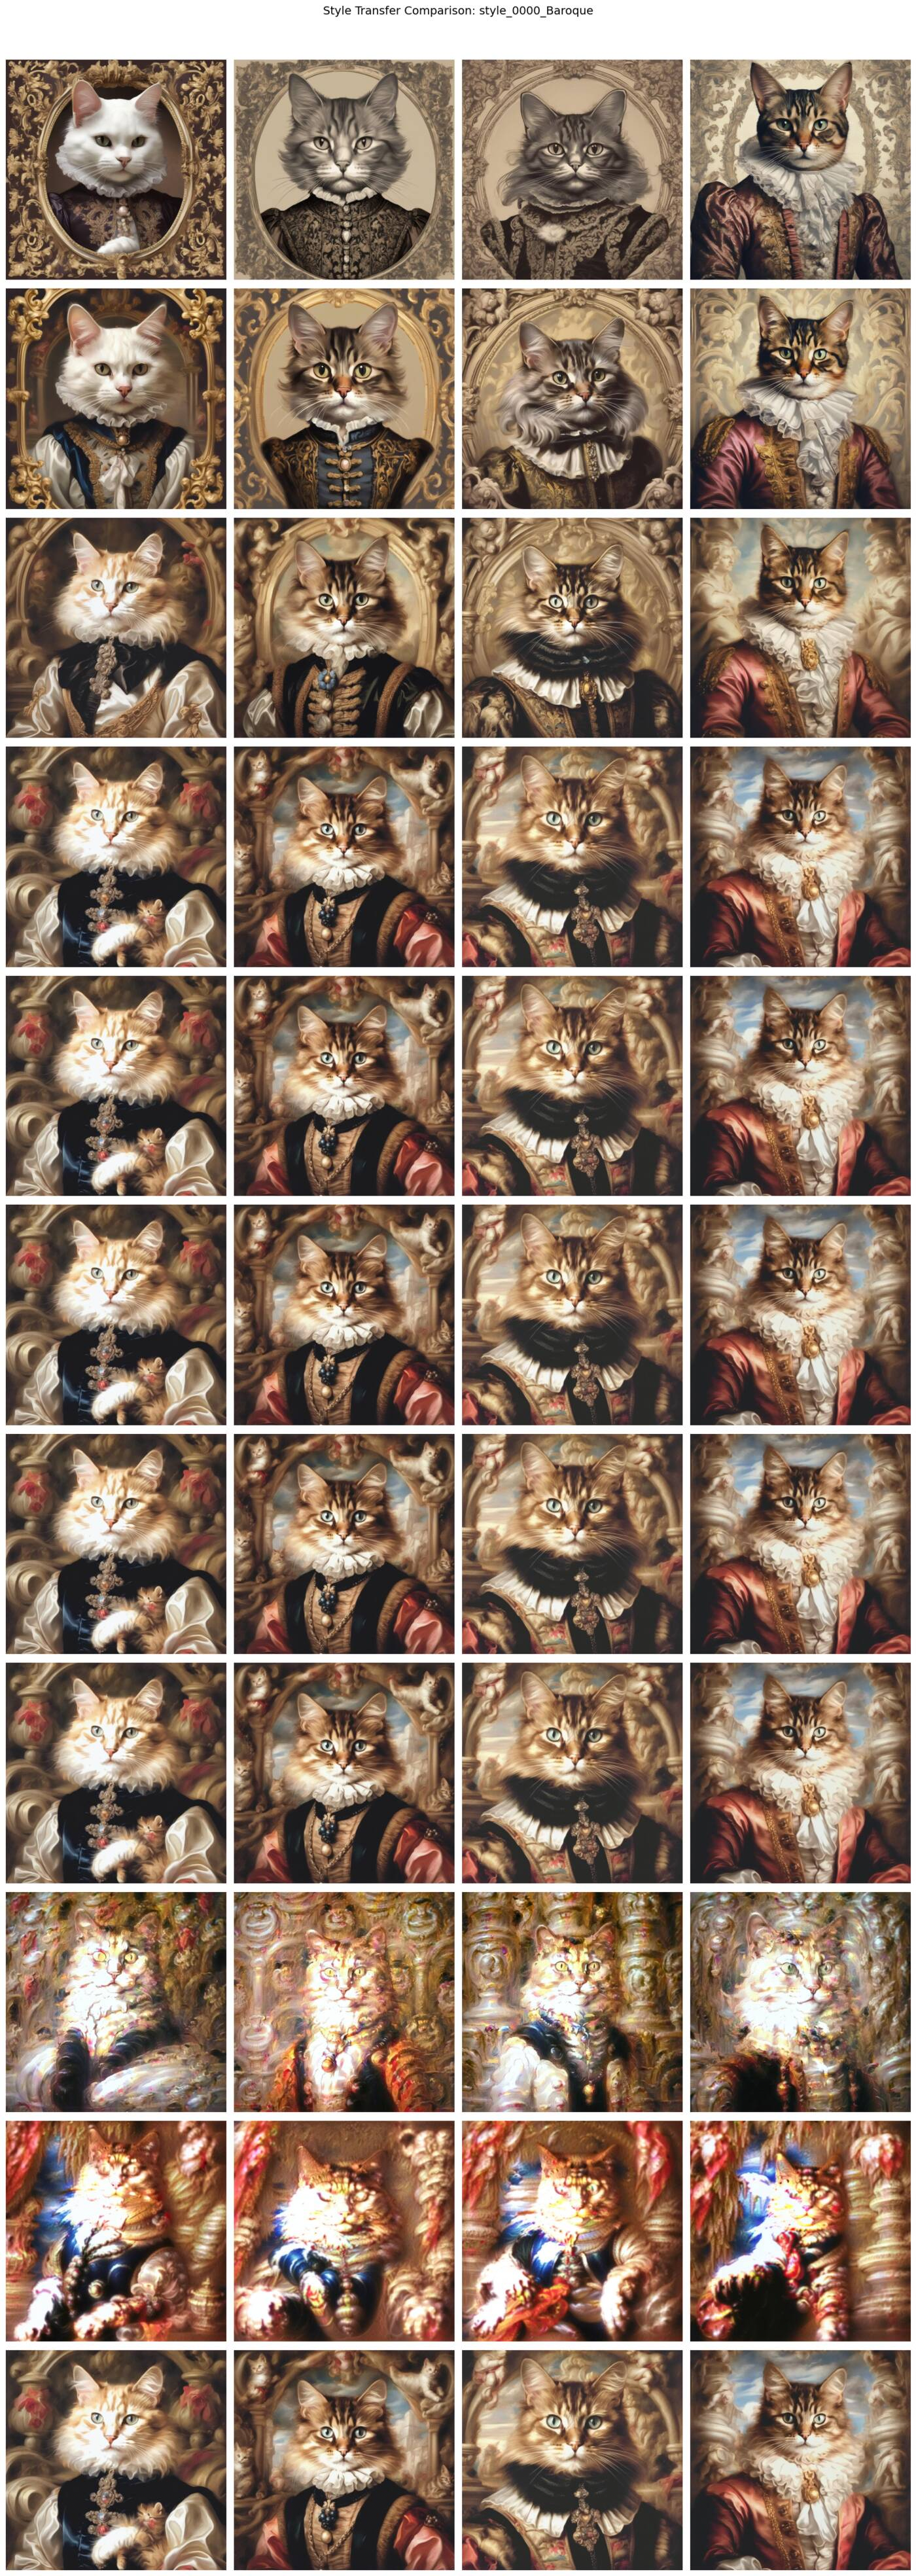
\includegraphics[width=\textwidth]{grid_Baroque.jpg}
    \column{0.32\textwidth}
      \centering \textbf{Cubism}\\[0.2em]
      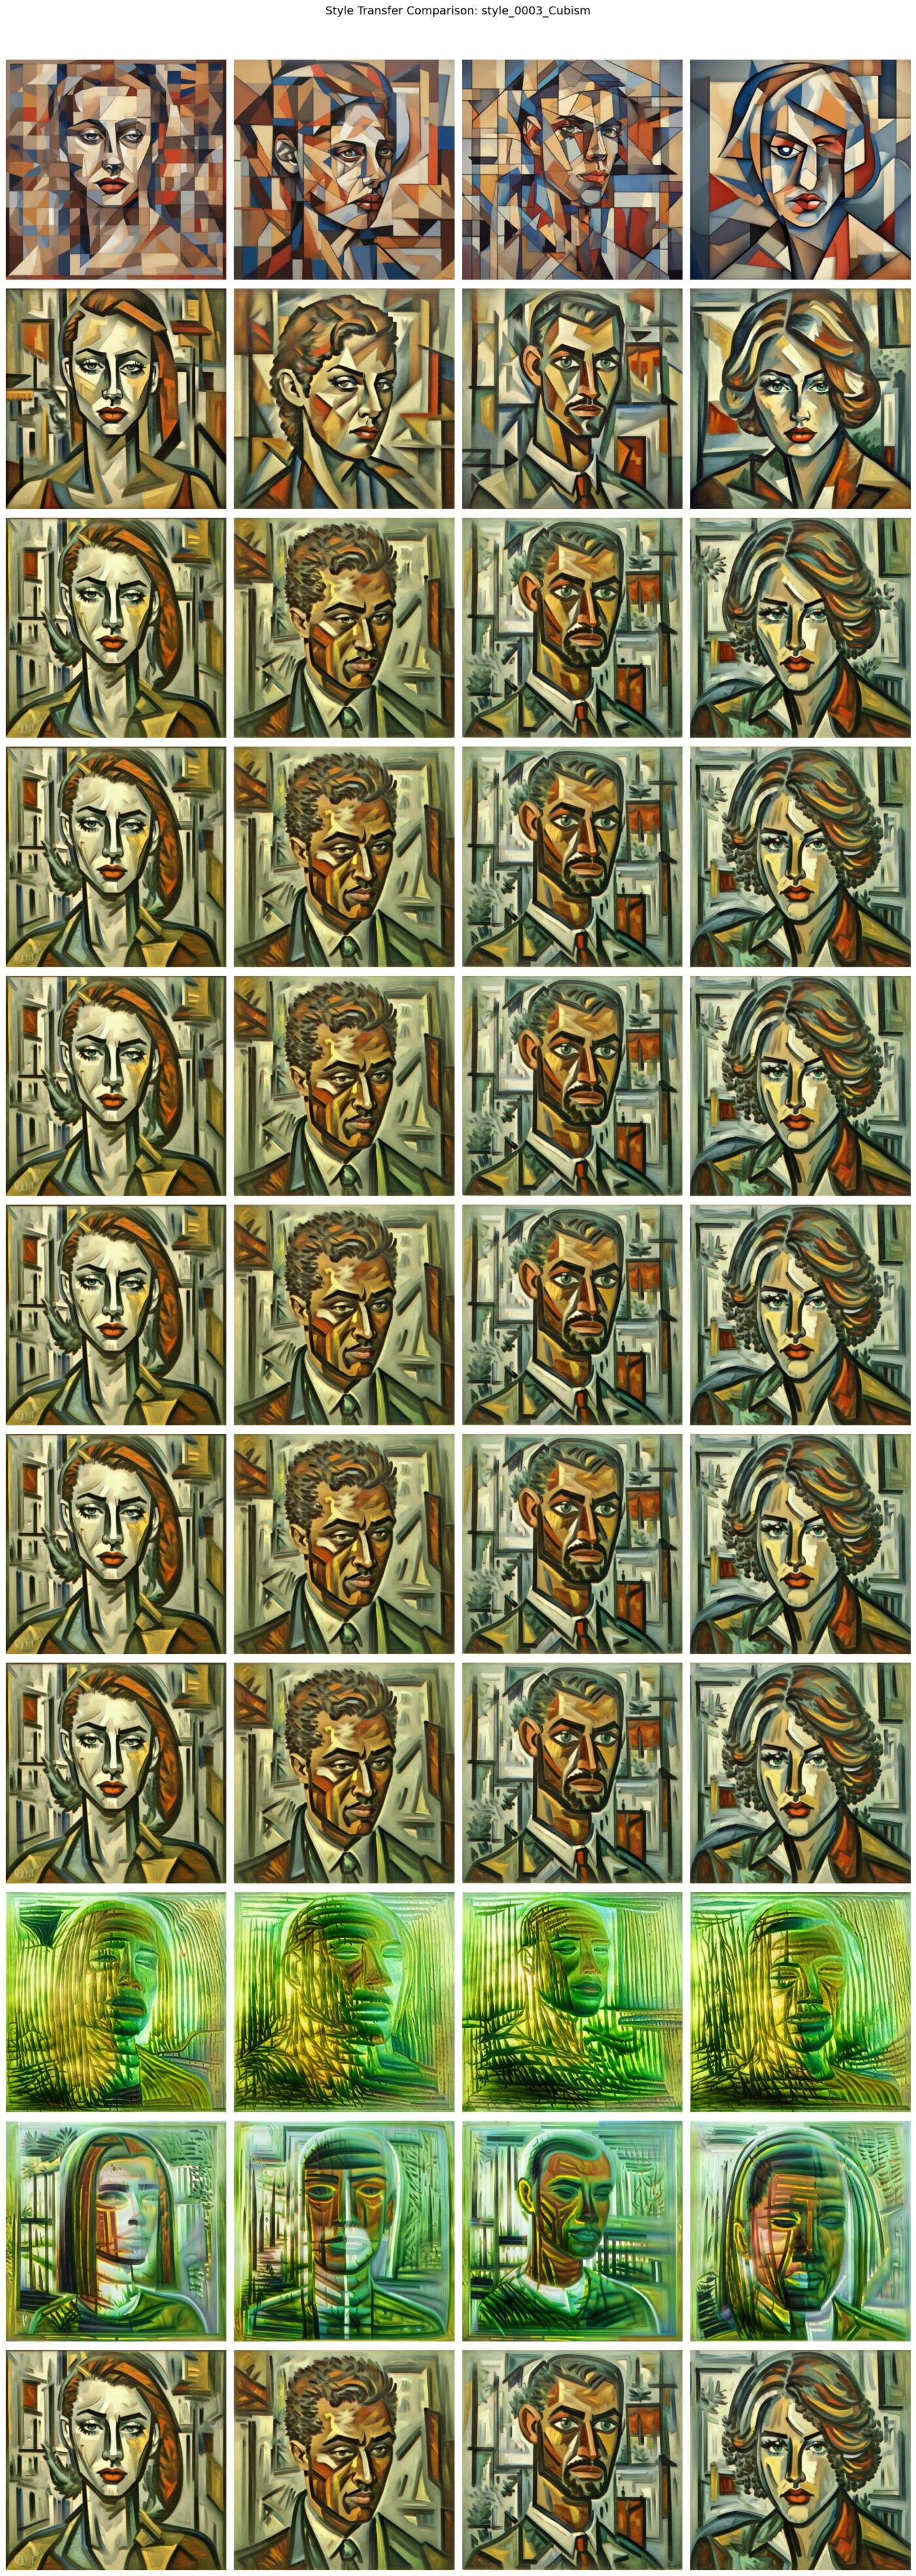
\includegraphics[width=\textwidth]{grid_Cubism.jpg}
    \column{0.32\textwidth}
      \centering \textbf{Expressionism}\\[0.2em]
      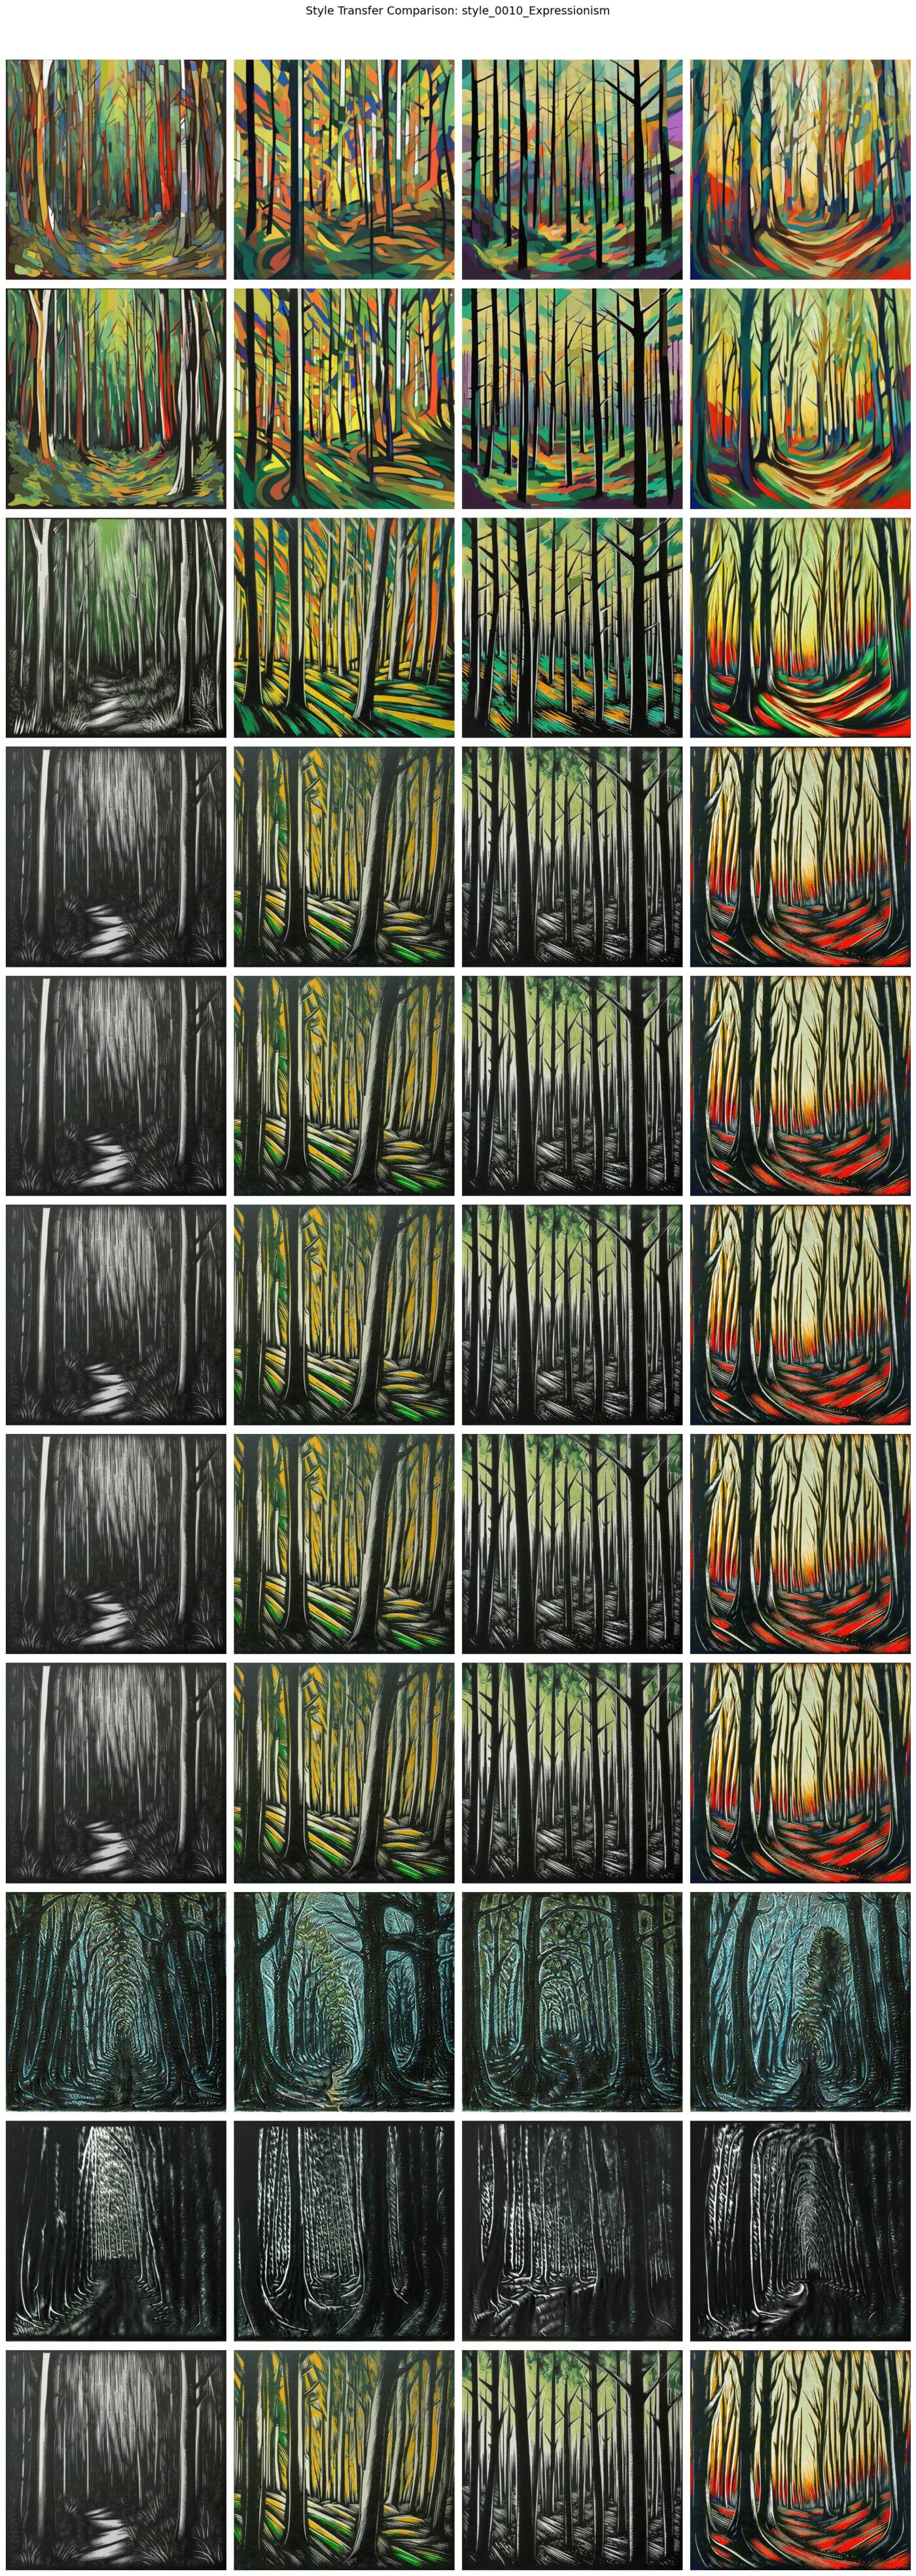
\includegraphics[width=\textwidth]{grid_Expressionism.jpg}
  \end{columns}
  \vspace{0.4em}
  \footnotesize Each grid: rows = routing configs ($\tau \in \{0.005, 0.05, 0.5\}$, $k \in \{1, \text{None}\}$) $\times$ cols = query images.
  Bottom row: reference B-LoRA (GT expert, oracle).
\end{frame}

%──────────────────────────────────────────────────────────────────────────────
\section{Model Variants Comparison}
%──────────────────────────────────────────────────────────────────────────────

\begin{frame}[shrink=10]{Model Variants Summary}
  \begin{center}
  \begin{tabular}{lcccccc}
    \toprule
    \textbf{Model} & \textbf{Stage} & \textbf{Loss} & \textbf{Steps} & \textbf{Synth.} & \textbf{$\alpha$} & \textbf{Status} \\
    \midrule
    v1.0 baseline & S1 & KL & 5k & naïve avg & 1.0 & \textcolor{darkgray}{obsolete} \\
    \midrule
    \textbf{S1 v2.0} (KL) & S1 & KL & 15,000 & product-sp. & 2.0 & \textcolor{mygreen}{\checkmark\ done} \\
    \textbf{S2 v2.0} (KL+LDM) & S2 & KL+LDM & 8,000 & product-sp. & 2.0 & \textcolor{mygreen}{\checkmark\ done} \\
    \textbf{S1 v2.1} (CE) & S1 & CE & 13,150 & product-sp. & 2.0 & \textcolor{mygreen}{\checkmark\ done} \\
    \textbf{S2 v2.1} (CE+LDM) & S2 & CE+LDM & --- & product-sp. & 2.0 & \textcolor{myorange}{training\ldots} \\
    \midrule
    \textit{Ref B-LoRA} & --- & --- & --- & GT LoRA & 1.0 & Oracle \\
    \bottomrule
  \end{tabular}
  \end{center}
  \vspace{0.5em}
  \begin{columns}[T]
    \column{0.48\textwidth}
      \begin{block}{Key design differences}
        \begin{itemize}
          \item \textbf{v2.0 vs v2.1}: training loss (KL vs CE); v2.1 uses hard one-hot GT, avoids noisy CLIP-similarity targets
          \item \textbf{S1 vs S2}: Stage 1 trains purely on routing; Stage 2 additionally closes the loop via SDXL denoising loss
        \end{itemize}
      \end{block}
    \column{0.48\textwidth}
      \begin{alertblock}{4-way comparison pending}
        Once S2 v2.1 training completes, we run the same 80-image sweep on all 4 checkpoints for a direct quality comparison.
      \end{alertblock}
  \end{columns}
\end{frame}

%──────────────────────────────────────────────────────────────────────────────
\section{Open Issues \& Next Steps}
%──────────────────────────────────────────────────────────────────────────────

\begin{frame}[shrink=15]{Open Issue: Prompt Mismatch}
  \begin{alertblock}{Critical unresolved problem}
    B-LoRA experts were trained with trigger token \texttt{"A [v]"}.\\
    Our inference sweeps use \emph{free-text} prompts like \texttt{"A Baroque painting"}.
  \end{alertblock}
  \vspace{0.5em}
  \begin{columns}[T]
    \column{0.50\textwidth}
      \begin{block}{Context}
        B-LoRA training (original work):
        \begin{itemize}
          \item Each expert fine-tuned on 30 images with prompt \texttt{"A [v]"}
          \item \texttt{[v]} is a \textbf{special learned token} embedded into SDXL's textual cross-attention
          \item At inference, \texttt{"A [v]"} activates the specific style representation
        \end{itemize}
      \end{block}
      \begin{block}{Our setup}
        \begin{itemize}
          \item We use prompts like \texttt{"A Baroque painting"},\\\texttt{"A painting in Cubist style"}, etc.
          \item SDXL text embeddings for these are \emph{completely different} from the token embedding \texttt{[v]}
          \item The LoRA weights may not activate optimally without the right trigger
        \end{itemize}
      \end{block}

    \column{0.47\textwidth}
      \begin{alertblock}{Impact}
        \begin{itemize}
          \item Style fidelity may be degraded even with correct routing
          \item Proper controlled experiment should use \texttt{"A [v]"} as prompt for all generated images
          \item Current results are a \textbf{lower bound} on achievable quality
        \end{itemize}
      \end{alertblock}
      \begin{exampleblock}{Proposed fix}
        \begin{enumerate}
          \footnotesize
          \item Run a parallel sweep using \texttt{"A [v]"} for all generations
          \item Compare: free-text prompt vs trigger token
          \item This isolates the prompt effect from the routing quality
        \end{enumerate}
      \end{exampleblock}
  \end{columns}
\end{frame}

\begin{frame}[shrink=15]{Engineering Challenges Overcome}
  \begin{columns}[T]
    \column{0.50\textwidth}
      \begin{block}{Challenge 1: O($N^2$) cross-term bug}
        \textbf{Symptom}: All inference outputs identical regardless of routing.\\
        \textbf{Root cause}: Naïve LoRA averaging introduces $O(N^2)$ cross-terms that cancel all style signal when $N$ is large.\\
        \textbf{Fix}: Product-space synthesis — compute $\bar{W}_t = \Sigma A_i W_i^\text{up} W_i^\text{down}$, then tSVD.
      \end{block}
      \vspace{0.3em}
      \begin{block}{Challenge 2: Alpha sub-threshold}
        \textbf{Symptom}: Correct routing, still identical images.\\
        \textbf{Root cause}: $\|\Delta W_\text{synth}\| \approx 16$ vs real B-LoRA $\approx 50$; at $\alpha=1.0$ only 32\% signal strength.\\
        \textbf{Fix}: Use $\alpha = 2.0$; also set \texttt{TARGET\_NORM=32} for \texttt{norm\_match} mode.
      \end{block}

    \column{0.47\textwidth}
      \begin{block}{Challenge 3: SVD numerical instability}
        \textbf{Three sub-issues}:
        \begin{enumerate}
          \footnotesize
          \item fp16 accumulation of $\bar{W}_t$ causes underflow/overflow in $N\!=\!109$ sum $\Rightarrow$ \textit{Fix}: accumulate in fp32
          \item cuSOLVER silently hangs on ill-conditioned matrices (no exception) $\Rightarrow$ \textit{Fix}: SVD on CPU (LAPACK)
          \item fp16 softmax NaN poisons the accumulation; noise retry also NaN $\Rightarrow$ \textit{Fix}: \texttt{nan\_to\_num} before SVD
        \end{enumerate}
      \end{block}
      \vspace{0.3em}
      \begin{alertblock}{Current status (job 765827 on ai12)}
        \footnotesize
        \textbf{Step 875/8000} --- running. LDM loss $\approx 0.55$ (improving).\\[0.2em]
        \textbf{Note}: \texttt{ent=-0.000000} --- entropy term not contributing.\\Attention distribution may be near-uniform (flat softmax).\\This is fix \#5; all previous SVD/NaN crashes now resolved.
      \end{alertblock}
  \end{columns}
\end{frame}

\begin{frame}[shrink=10]{Next Steps}
  \begin{columns}[T]
    \column{0.50\textwidth}
      \begin{block}{Immediate (days)}
        \begin{enumerate}
          \item Confirm Stage 2 v2.1 (CE+LDM) training succeeds
          \item Run inference sweep on S2 v2.1 ($\alpha=2.0$)
          \item \textbf{4-way comparison}: S1v2.0 / S2v2.0 / S1v2.1 / S2v2.1
        \end{enumerate}
      \end{block}
      \vspace{0.5em}
      \begin{block}{Short-term (week)}
        \begin{enumerate}
          \item Controlled experiment: \texttt{"A [v]"} prompt vs free-text
          \item Qualitative evaluation using CLIP-style similarity metric
          \item Ablation: temperature, top-$k$ effect
        \end{enumerate}
      \end{block}

    \column{0.47\textwidth}
      \begin{block}{Medium-term}
        \begin{enumerate}
          \item Quantitative metrics: FID, LPIPS, style CLIP-similarity
          \item Multi-style queries (interpolation between styles)
          \item Out-of-distribution testing (styles not in zoo)
          \item Potential: joint fine-tuning of encoder + minimal LoRA layers
        \end{enumerate}
      \end{block}
      \vspace{0.3em}
      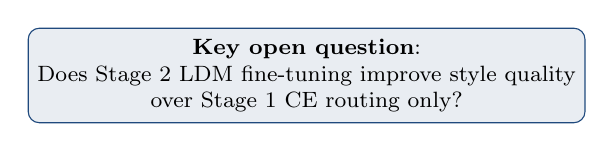
\begin{tikzpicture}
        \node[draw=myblue,fill=myblue!10,rounded corners,minimum width=5cm,minimum height=1.2cm,align=center,font=\footnotesize] {%
          \textbf{Key open question}:\\
          Does Stage 2 LDM fine-tuning improve style quality\\over Stage 1 CE routing only?
        };
      \end{tikzpicture}
  \end{columns}
\end{frame}

%──────────────────────────────────────────────────────────────────────────────
\section{Summary}
%──────────────────────────────────────────────────────────────────────────────

\begin{frame}[shrink=10]{Summary}
  \begin{columns}[T]
    \column{0.50\textwidth}
      \begin{exampleblock}{What we built}
        \begin{itemize}
          \item \textbf{MoELoRA v2}: per-tensor rank-level attention router over 109 B-LoRA style experts
          \item \textbf{LoRARankEncoder} (2.2M params): shared point-wise MLP encoding LoRA rows to key vectors
          \item \textbf{Product-space synthesis} + tSVD: correct, numerically stable multi-expert blending
          \item \textbf{Two-stage training}: CE routing (S1) + LDM denoising loop (S2)
        \end{itemize}
      \end{exampleblock}
      \begin{block}{Key findings}
        \begin{itemize}
          \item Routing \textbf{is working} (non-uniform heatmaps, semantically relevant top-$k$)
          \item $\alpha=2.0$ is the sweet spot for visible, non-distorted style injection
          \item CE loss (v2.1) gives cleaner routing targets than KL
        \end{itemize}
      \end{block}

    \column{0.47\textwidth}
      \begin{alertblock}{Open challenges}
        \begin{itemize}
          \item Prompt mismatch: \texttt{"A [v]"} vs free-text
          \item Stage 2 SVD stability (fp16 training, 4 attempts)
          \item No quantitative evaluation yet
        \end{itemize}
      \end{alertblock}
      \vspace{0.5em}
      \begin{block}{Completed experiments}
        \begin{itemize}
          \item[$\checkmark$] S1 v2.0 sweep: 80 images
          \item[$\checkmark$] S1 v2.1 sweep: 80 images
          \item[$\checkmark$] S2 v2.0 sweep: 80 images
          \item[$\checkmark$] Alpha diagnostic: 12 configurations
          \item[\ldots] S2 v2.1: training in progress
        \end{itemize}
      \end{block}
  \end{columns}
\end{frame}

%──────────────────────────────────────────────────────────────────────────────
\appendix
%──────────────────────────────────────────────────────────────────────────────

\begin{frame}{Appendix: Complete Model Architecture}
  \begin{center}
  \resizebox{0.95\textwidth}{!}{
  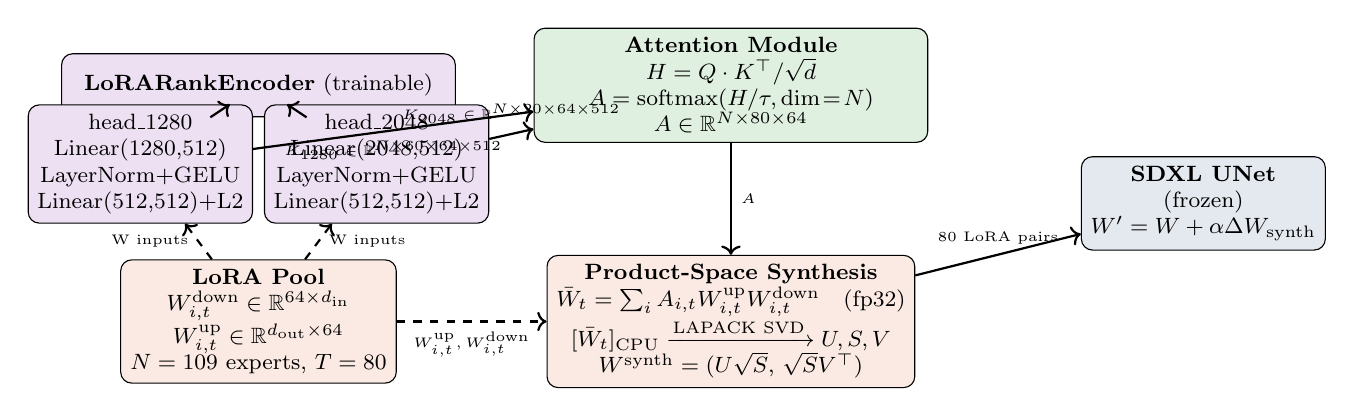
\begin{tikzpicture}[
    arr/.style={->,thick},
  ]
  \node[detbox=mypurple,minimum width=5cm] (enc_title) at (0,3) {\textbf{LoRARankEncoder} (trainable)};
  \node[detbox=mypurple,minimum width=2.2cm] (h1280) at (-1.5,2) {head\_1280\\Linear(1280,512)\\LayerNorm+GELU\\Linear(512,512)+L2};
  \node[detbox=mypurple,minimum width=2.2cm] (h2048) at (1.5,2) {head\_2048\\Linear(2048,512)\\LayerNorm+GELU\\Linear(512,512)+L2};
  \draw[arr] (enc_title) -- (h1280);
  \draw[arr] (enc_title) -- (h2048);

  % Attention
  \node[detbox=mygreen,minimum width=5cm] (attn) at (6,3) {\textbf{Attention Module}\\$H = Q \cdot K^\top / \sqrt{d}$\\$A = \text{softmax}(H/\tau, \dim\!=\!N)$\\$A \in \RR^{N \times 80 \times 64}$};
  \draw[arr] (h1280) -- node[below,font=\tiny]{$K_\text{1280} \in \RR^{N\times 60\times 64\times 512}$} (attn);
  \draw[arr] (h2048) -- node[above,font=\tiny]{$K_\text{2048} \in \RR^{N\times 20\times 64\times 512}$} (attn);

  % Pool
  \node[detbox=myorange,minimum width=3.5cm] (pool) at (0,0) {\textbf{LoRA Pool}\\$W^\text{down}_{i,t} \in \RR^{64\times d_\text{in}}$\\$W^\text{up}_{i,t} \in \RR^{d_\text{out}\times 64}$\\$N=109$ experts, $T=80$};
  \draw[arr,dashed] (pool) -- node[left,font=\tiny]{W inputs} (h1280);
  \draw[arr,dashed] (pool) -- node[right,font=\tiny]{W inputs} (h2048);

  % Synthesis
  \node[detbox=myorange,minimum width=4.5cm] (synth) at (6,0) {\textbf{Product-Space Synthesis}\\$\bar{W}_t = \sum_i A_{i,t} W^\text{up}_{i,t} W^\text{down}_{i,t}$\quad (fp32)\\$[\bar{W}_t]_\text{CPU} \xrightarrow{\text{LAPACK SVD}} U,S,V$\\$W^\text{synth} = (U\sqrt{S},\, \sqrt{S}V^\top)$};
  \draw[arr] (attn) -- node[right,font=\tiny]{$A$} (synth);
  \draw[arr,dashed] (pool) -- node[below,font=\tiny]{$W^\text{up}_{i,t}, W^\text{down}_{i,t}$} (synth);

  % SDXL
  \node[detbox=myblue,minimum width=3cm] (sdxl) at (12,1.5) {\textbf{SDXL UNet}\\(frozen)\\$W' = W + \alpha \Delta W_\text{synth}$};
  \draw[arr] (synth) -- node[above,font=\tiny]{80 LoRA pairs} (sdxl);
  \end{tikzpicture}
  }
  \end{center}
\end{frame}

\begin{frame}[shrink=10]{Appendix: Oracle Test --- Synthesis Fidelity}
  \begin{columns}[T]
    \column{0.55\textwidth}
      \begin{block}{Oracle routing experiment}
        Set attention weight 1.0 on GT expert, 0.0 on all others.\\
        Product-space synthesis should recover the GT LoRA exactly.
        \[
          A_\text{oracle} = e_g \quad\Rightarrow\quad \bar{W}_t = W^\text{up}_{g,t} W^\text{down}_{g,t}
        \]
        SVD of a rank-$r$ matrix:
        \[
          W^\text{up}_{g,t} W^\text{down}_{g,t} \xrightarrow{\text{tSVD}} W^\text{up}_\text{synth}, W^\text{down}_\text{synth}
        \]
      \end{block}
      \begin{exampleblock}{Measured result}
        \[
          \cos\!\left(W^\text{up}_\text{synth} W^\text{down}_\text{synth},\; W^\text{up}_g W^\text{down}_g\right) = \mathbf{0.9998}
        \]
        $\Rightarrow$ synthesis is numerically lossless at oracle.\\[0.3em]
        \footnotesize (Small error from float32 SVD truncation at rank 64)
      \end{exampleblock}

    \column{0.42\textwidth}
      \includegraphics[width=\textwidth]{alpha_diag/synth_oracle_a3.0/synth_oracle_a3.0_A_Baroque_painting_0.jpg}
      \vspace{0.3em}\\
      \footnotesize Oracle output ($\alpha=3.0$): clear content leakage from top-1 expert confirms injection is working.
  \end{columns}
\end{frame}

\begin{frame}[shrink=15]{Appendix: Training Configuration}
  \begin{columns}[T]
    \column{0.50\textwidth}
      \begin{block}{Stage 1 hyperparameters}
        \begin{tabular}{lll}
          \toprule
          & v2.0 (KL) & v2.1 (CE) \\
          \midrule
          Loss & KL div & Cross-Entropy \\
          Max steps & 15,000 & 15,000 \\
          LR & 3e-4 & 3e-4 \\
          Warmup & 500 & 500 \\
          LR sched. & cosine & cosine \\
          Batch size & 8 & 8 \\
          Pool size & 5–20 & 5–20 \\
          $\tau$ label & 0.3 & --- \\
          Grad clip & 1.0 & 1.0 \\
          \bottomrule
        \end{tabular}
      \end{block}

    \column{0.47\textwidth}
      \begin{block}{Stage 2 hyperparameters}
        \begin{tabular}{ll}
          \toprule
          Param & Value \\
          \midrule
          Max steps & 8,000 \\
          LR & 5e-5 \\
          Warmup & 200 \\
          Precision & fp16 mixed \\
          $\lambda_\text{ent}$ & $0.1 \to 0.01$ \\
          Batch size & 1 \\
          Pool size & 5–20 (no GT) \\
          LoRA $\alpha$ & 1.0 (training) \\
          \bottomrule
        \end{tabular}
      \end{block}
      \begin{block}{Hardware}
        VALAR HPC $\cdot$ NVIDIA A100 GPU\\
        SLURM scheduling $\cdot$ 24h time limit
      \end{block}
  \end{columns}
\end{frame}

%──────────────────────────────────────────────────────────────────────────────
\begin{frame}[plain]
  \begin{center}
    \LARGE\textbf{Thank You}\\[1em]
    \large Questions?\\[2em]
    \normalsize
    \textcolor{myblue}{Code:} \texttt{MoLoRAs/lora\_attention/}\\[0.3em]
    \textcolor{myblue}{Results:} \texttt{/scratch/eyavuz21/lora\_attention/}\\[0.3em]
    \textcolor{myblue}{Roadmap:} \texttt{lora\_attention/roadmap.md}
  \end{center}
\end{frame}
%──────────────────────────────────────────────────────────────────────────────

\end{document}
